% book example for classicthesis.sty
\documentclass[
  % Replace twoside with oneside if you are printing your thesis on a single side
  % of the paper, or for viewing on screen.
  %oneside,
  oneside,
  11pt, a4paper,
  footinclude=true,
  headinclude=true,
  cleardoublepage=empty
]{scrbook}

\tolerance=100
\usepackage{lipsum}
\usepackage[hidelinks]{hyperref}
\usepackage{graphicx}
\usepackage[linedheaders,parts,pdfspacing]{classicthesis}
\usepackage{acronym}
\usepackage{microtype}
\usepackage[british]{babel}

\usepackage{float}
\usepackage{caption}
\usepackage{subcaption}
\usepackage{gensymb}

\usepackage{amsmath,amsfonts,amsthm,amssymb}
\usepackage[cal=cm]{mathalfa}

\newtheorem{mydef}{Definition}
\newtheorem{myprop}{Property}
\newtheorem{mythm}{Theorem}
\newtheorem{mylem}{Lemma}

\graphicspath{{./Figures/}}


\title{Penrose Aperiodic Tiling of the Plane and Graphical Geodesics}
\author{Jesse Bettencourt\\1144386\\[80pt]  \textit{Supervisor: Dr. Miroslav Lovric}}

\begin{document}
\section{Up-Down Construction}

In his 1990 paper \textit{Updown generation of Penrose patterns}, de Bruijn describes a construction method attributed to Conway by which tilings are generated by infinite sequences of steps along a directed graph. The Up-Down generation process borrows some concepts from the substitution method, namely that we build tilings by substituting tiles with constituent decomposition tiles, as per substitution rules. The key difference, however, is that we build a tiling instead by considering the relationship between a constituent tile and its inflation. As the name suggests, Up-Down generation constructs tilings through two processes: Up and Down.

In introducing this construction method, we must consider again the Robinson triangles. As with the substitution method, decomposition of these triangles is dependent on their orientation. Unlike substitution, the influence of triangle orientation under the Up-Down method is subtle and not automatic. Moving forward, we must be explicit with the triangle orientation, see Fig.\ref{fig:OrientedRob}.

 

\begin{figure}[h]
        \begin{subfigure}[t]{0.4\textwidth}
                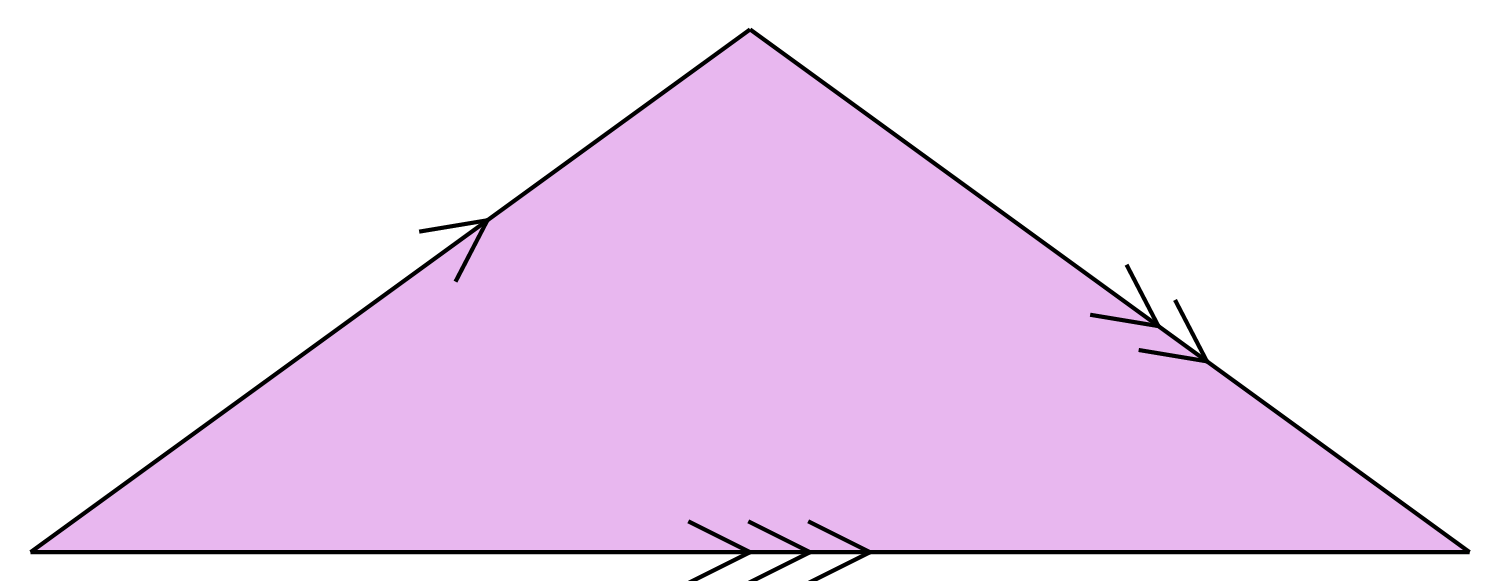
\includegraphics[width=\textwidth]{TFRob}
                \caption*{\Large T}
        \end{subfigure}\hfill
        \begin{subfigure}[t]{0.3\textwidth}
                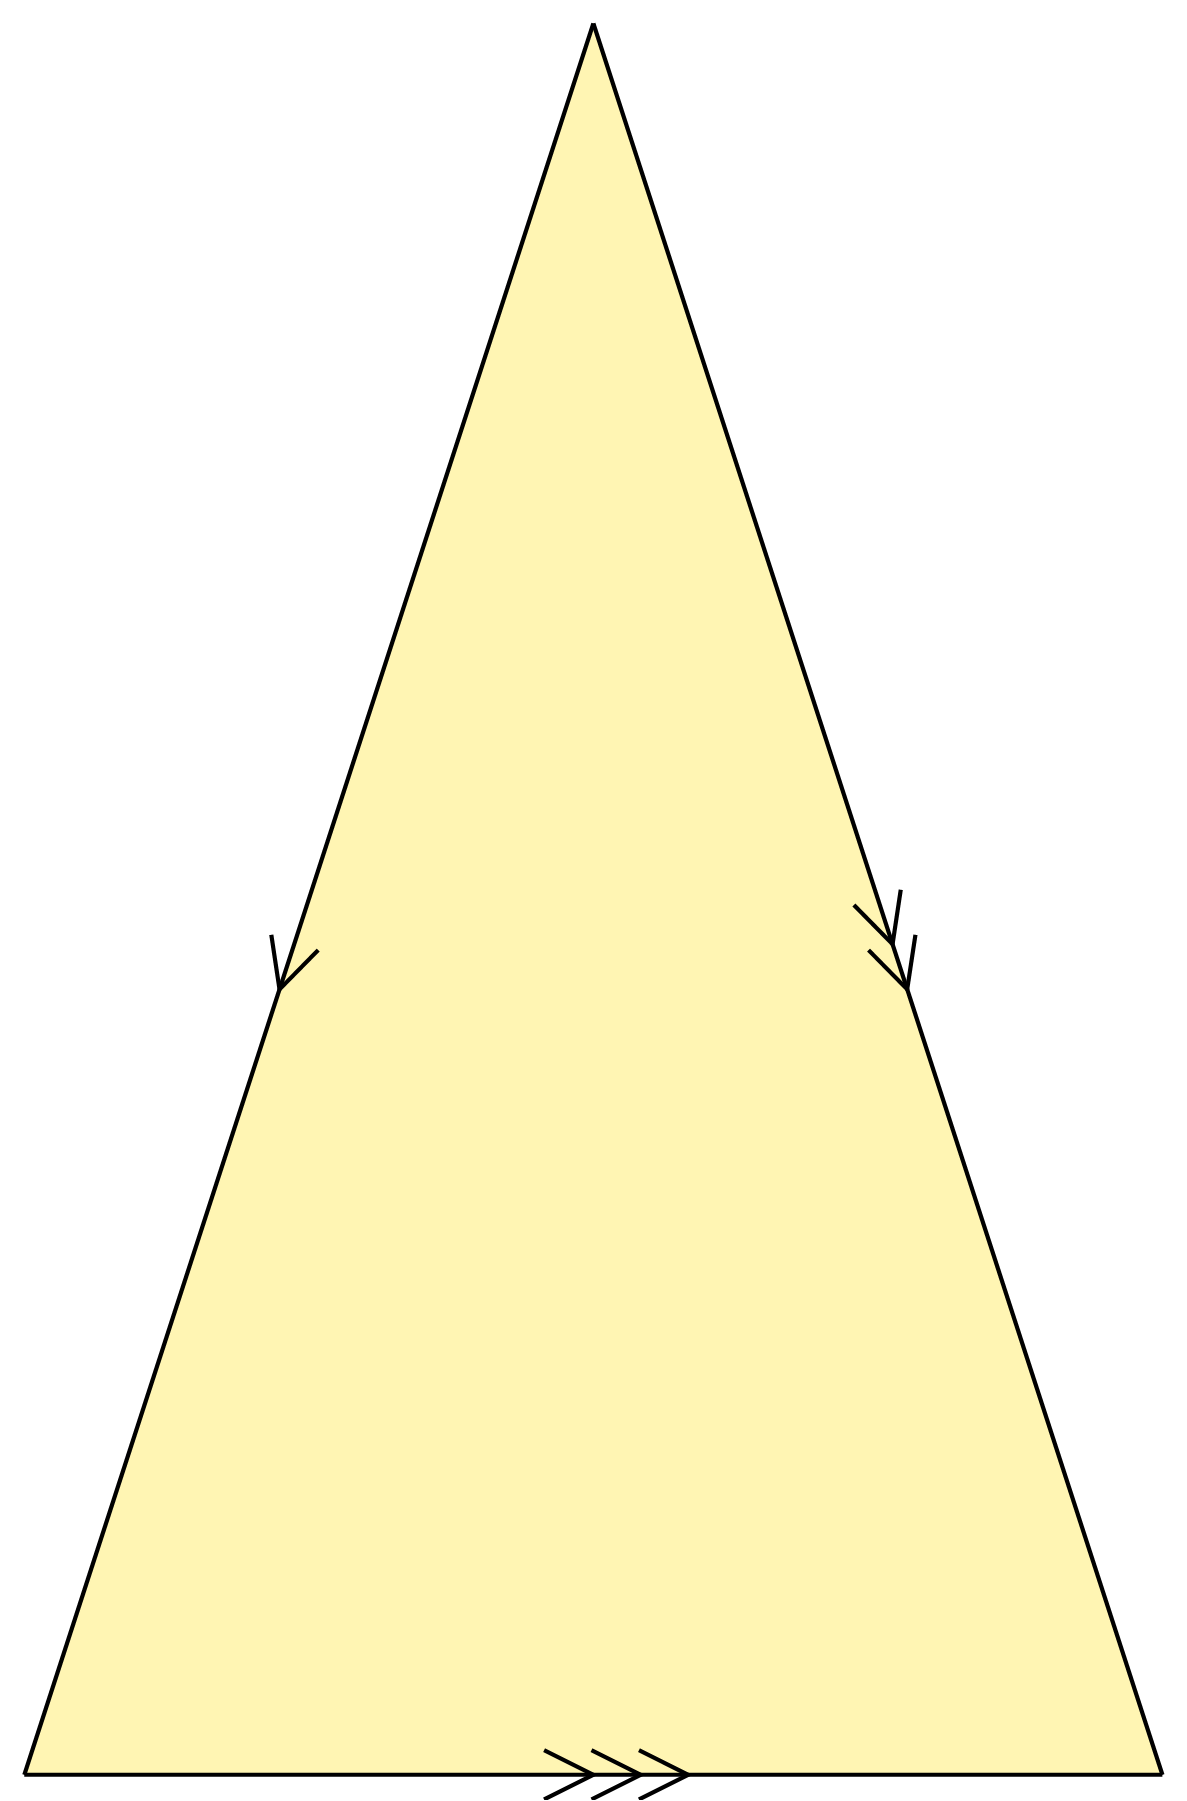
\includegraphics[width=\textwidth]{TSRob}
                \caption*{\Large t}
        \end{subfigure}\\
        
        \begin{subfigure}[t]{0.4\textwidth}
                \raisebox{0px}{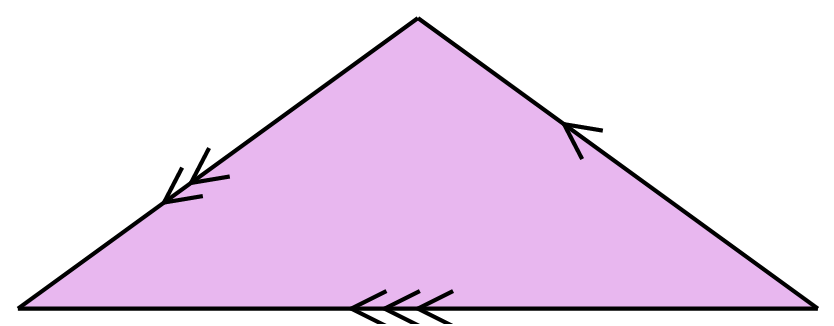
\includegraphics[width=\textwidth]{T'FRob}}
                \caption*{\Large T'}
        \end{subfigure}\hfill
        \begin{subfigure}[t]{0.3\textwidth}
                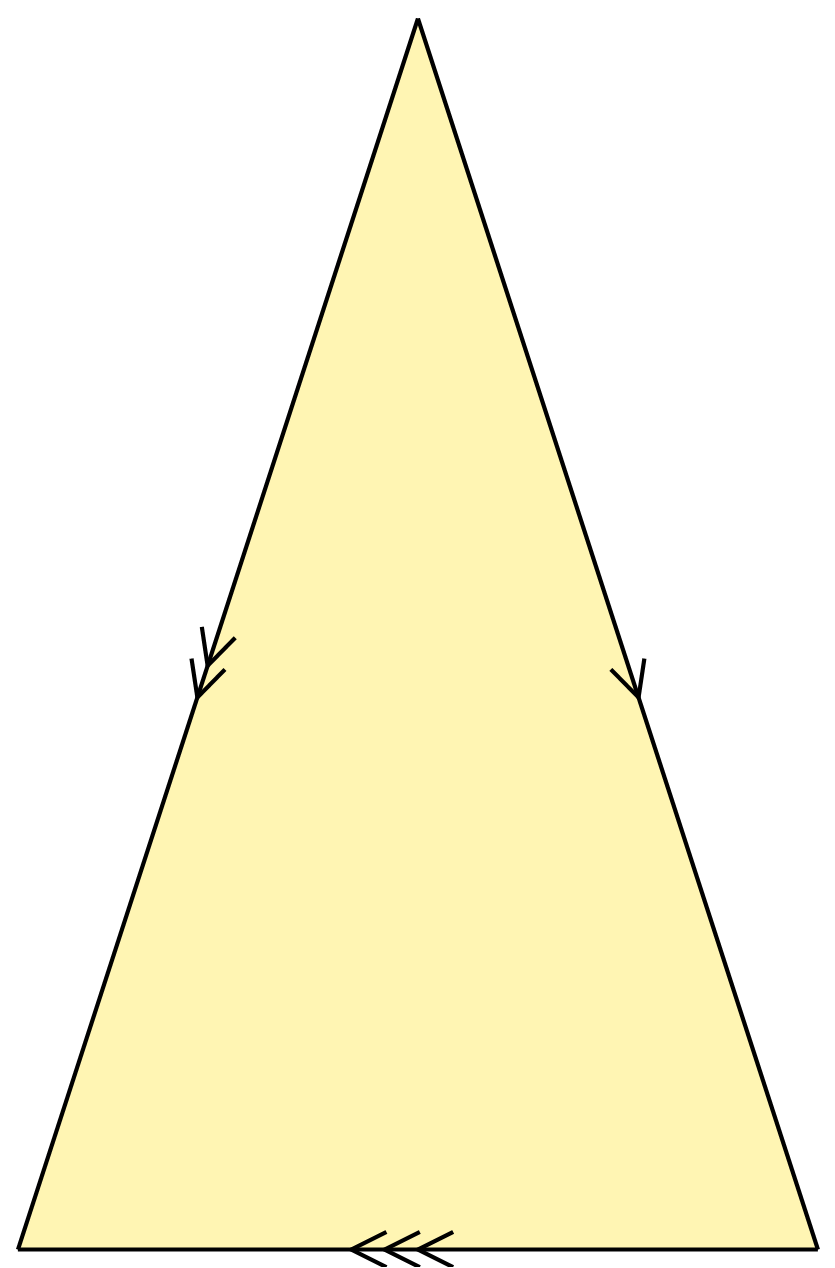
\includegraphics[width=\textwidth]{T'SRob}
                \caption*{\Large t'}
        \end{subfigure}  
        \caption{Oriented Robinson triangles. Thick or Obtuse Robinson Triangle is denoted with T. Thin or acute Robinson triangle is denoted with t. Reversed orientation is denoted with '. Arrowed edges illustrate Up-Down matching rules.}  
        \label{fig:OrientedRob}                    
\end{figure}

The matching rules under the substitution method behave slightly differently than the matching rules in the Up-Down method, illustrated with arrowed edges in Fig.\ref{fig:OrientedRob}. Here, the rules will indicate type and direction of edges, which must agree along abutting tiles. Additionally, the edge type and direction will satisfy decomposition rules according to the relationship between a triangle and it's constituent triangles, see Fig.\ref{fig:EdgeRules}. 

\begin{figure}[H]
        \begin{subfigure}[t]{0.4\textwidth}
                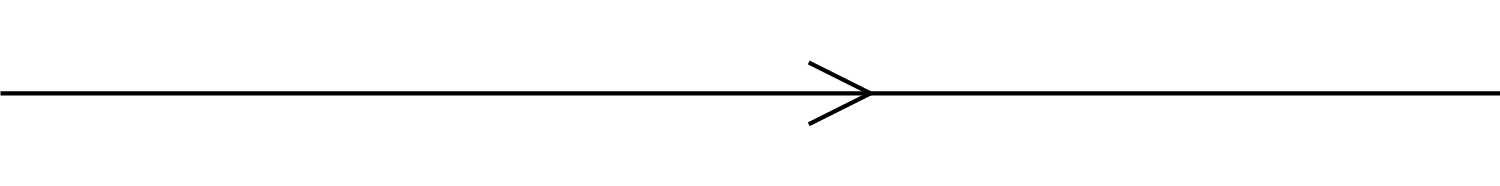
\includegraphics[width=\textwidth]{a1}
        \end{subfigure}\hfill
        \begin{subfigure}[t]{0.4\textwidth}
                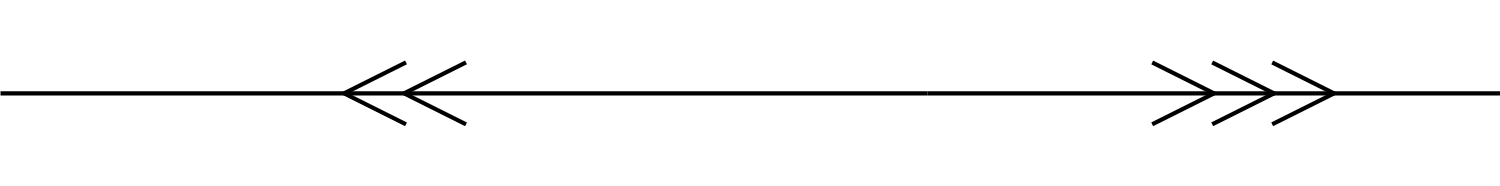
\includegraphics[width=\textwidth]{a1inflate}
        \end{subfigure}\\
        
        \begin{subfigure}[t]{0.4\textwidth}
                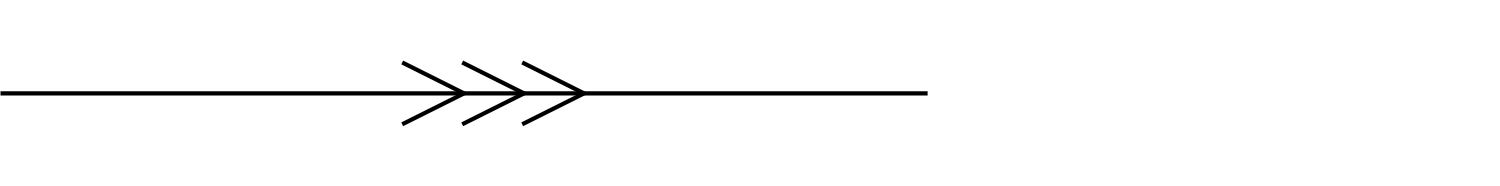
\includegraphics[width=\textwidth]{a2}
        \end{subfigure}\hfill
        \begin{subfigure}[t]{0.4\textwidth}
                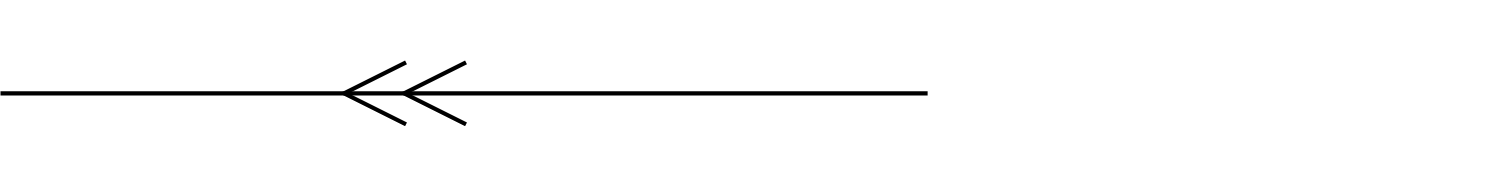
\includegraphics[width=\textwidth]{a2inflate}
        \end{subfigure}\\    
        
        \begin{subfigure}[t]{0.4\textwidth}
                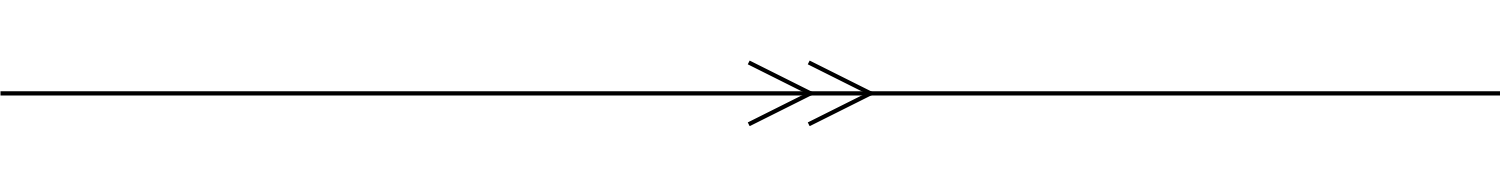
\includegraphics[width=\textwidth]{a3}
        \end{subfigure}\hfill
        \begin{subfigure}[t]{0.4\textwidth}
                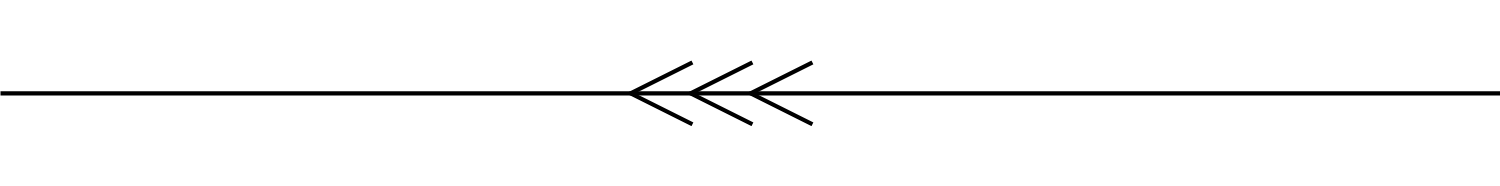
\includegraphics[width=\textwidth]{a3inflate}
        \end{subfigure}\\                           
        
        \begin{subfigure}[t]{0.4\textwidth}
                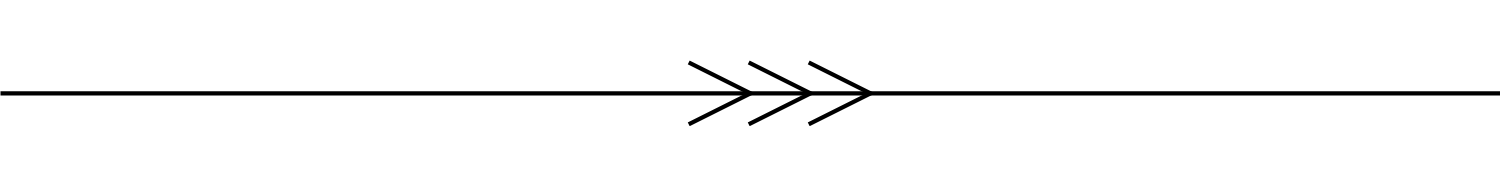
\includegraphics[width=\textwidth]{a4}
        \end{subfigure}\hfill
        \begin{subfigure}[t]{0.4\textwidth}
                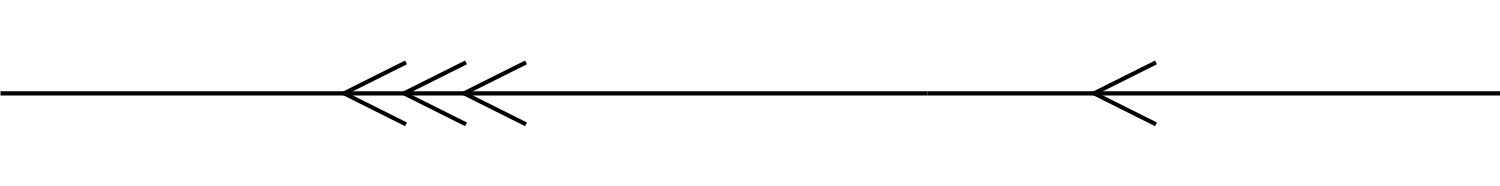
\includegraphics[width=\textwidth]{a4inflate}
        \end{subfigure}\\   
        \caption{Parent edges (Left) and their constituent edges (Right)}     
        \label{fig:EdgeRules}
\end{figure} 


\pagebreak
Consider again the substitution rules on the Robinson triangles described in Fig.\ref{fig:RobSubs}. This substitution is also employed in the Up-Down method. However, in this case we will label the constituent triangles of the substitution. We do this so we can explicitly describe the relationship between a constituent triangle and its parent triangle. We label this relationship using mapping functions, given by lowercase Greek letters: $\alpha, \beta, \delta, \gamma$. We see the oriented Robinson triangles, substituted with relationship labels, in Fig.\ref{fig:OrientedSub}.

These relationship labels can be considered as mappings from a constituent triangle to its parent triangle. These mappings are as follows:
\begin{align}
\epsilon &: T \rightarrow T  &\epsilon' &: T' \rightarrow T' \nonumber\\  
\alpha &: T \rightarrow t  &\alpha' &: T' \rightarrow t' \nonumber\\  
\beta &: t \rightarrow t  &\beta' &: t' \rightarrow t' \label{eq:maps}\\  
\delta &: t' \rightarrow T  &\delta' &: t \rightarrow T' \nonumber\\ 
\gamma &: T' \rightarrow T  &\gamma' &: T \rightarrow T' \nonumber
\end{align}
Again, these mappings are also labeled in Fig.\ref{fig:OrientedSub}. For an example of how to interpret this mapping, consider the mapping $\delta$ which maps constituent \textbf{t'} to parent \textbf{T}. This tells us that following relationship $\delta$, the yellow \textbf{t'} triangle will be located inside the pink \textbf{T} parent.



\begin{figure}[H]
        \begin{subfigure}[t]{0.55\textwidth}
                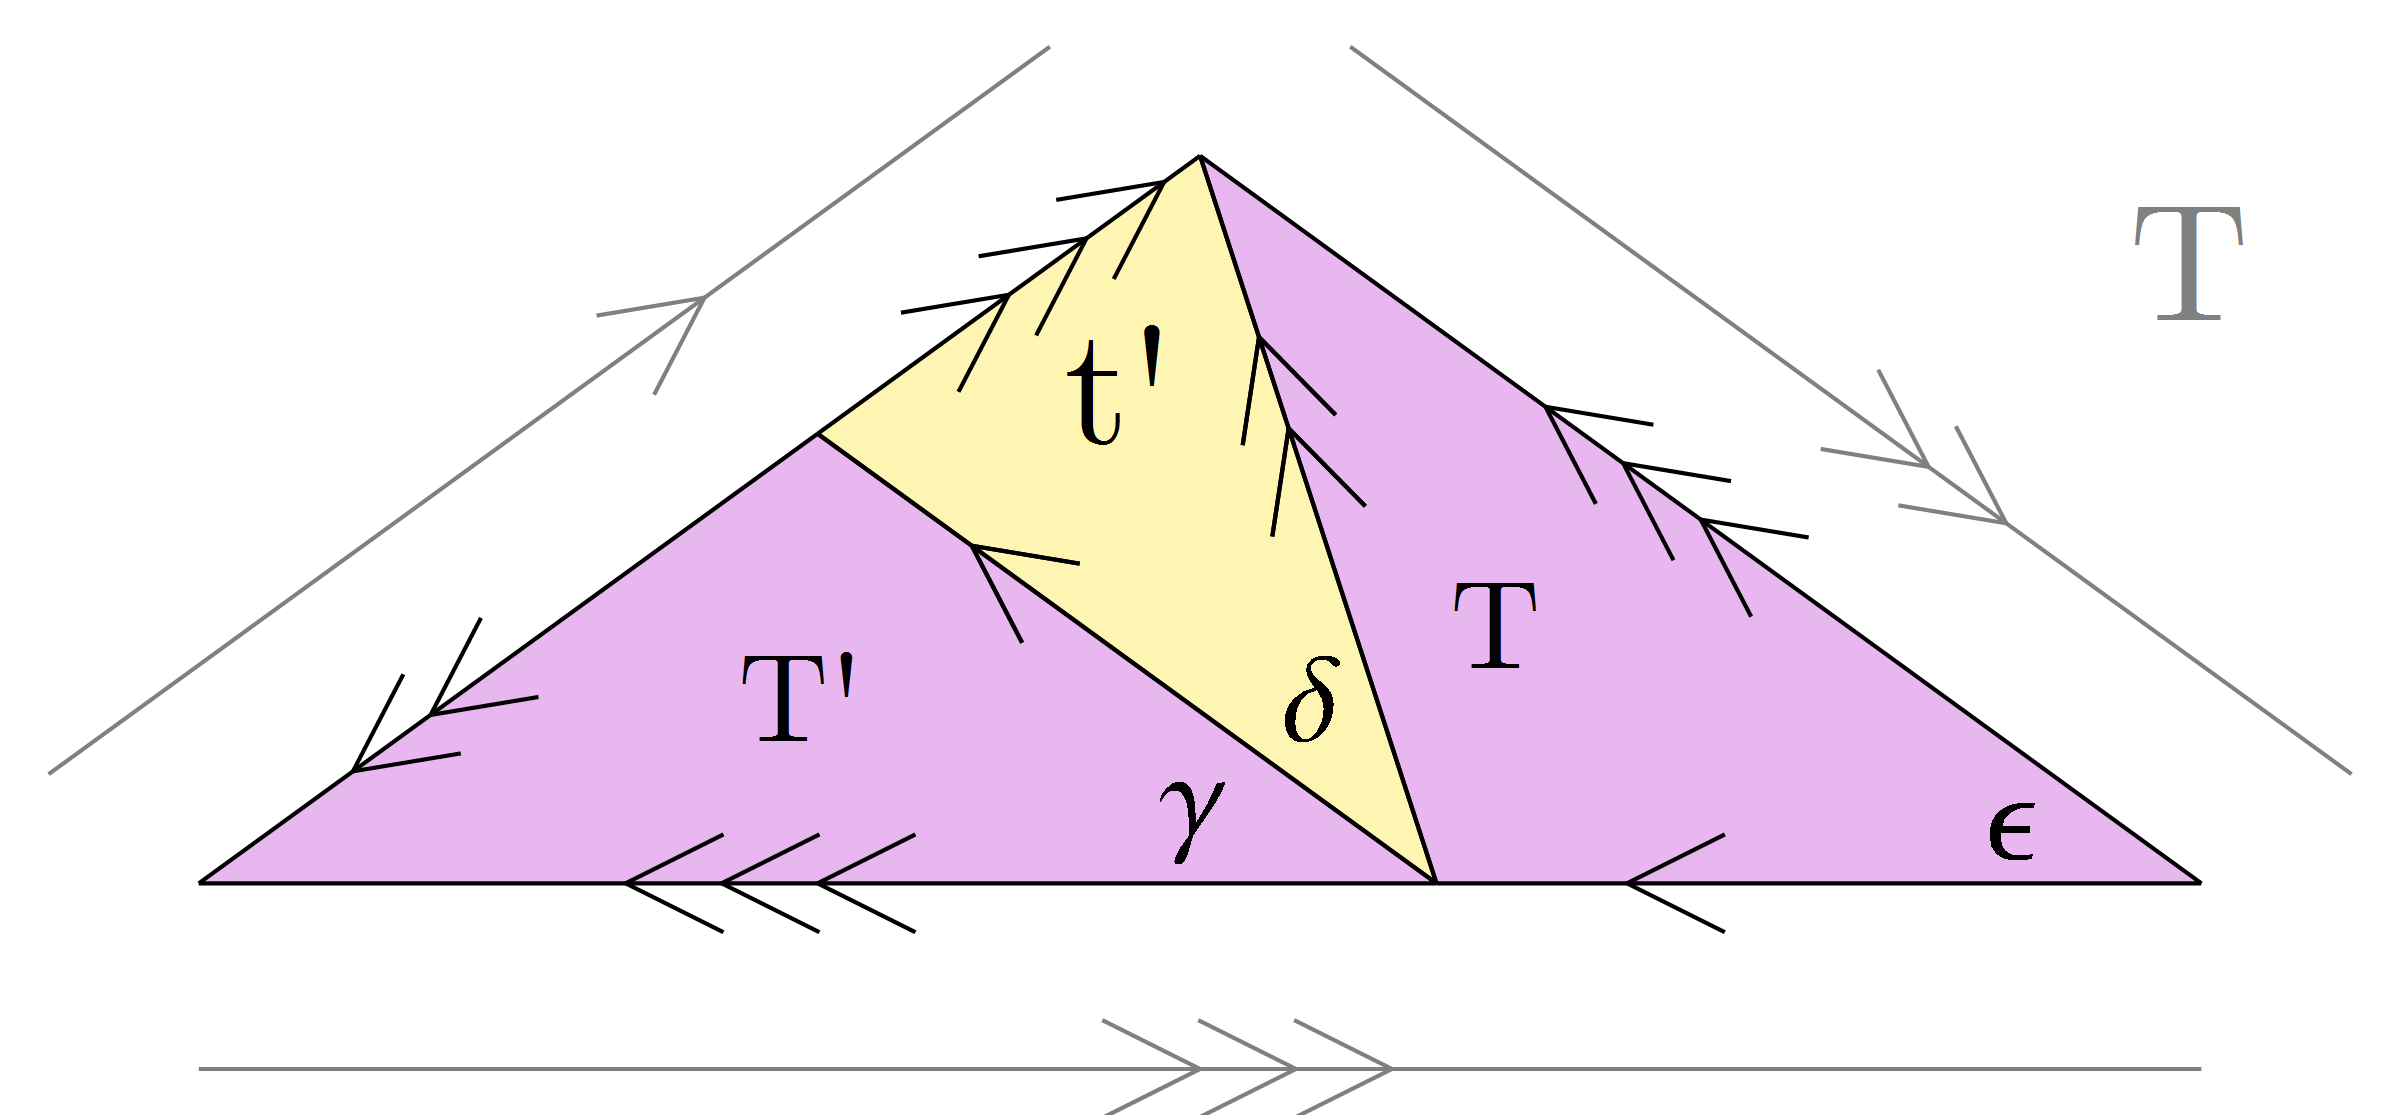
\includegraphics[width=\textwidth]{TF}
        \end{subfigure}\hfill
        \begin{subfigure}[t]{0.35\textwidth}
                \includegraphics[width=\textwidth]{TS}
        \end{subfigure}\\
        
        \begin{subfigure}[t]{0.55\textwidth}
                \raisebox{55px}{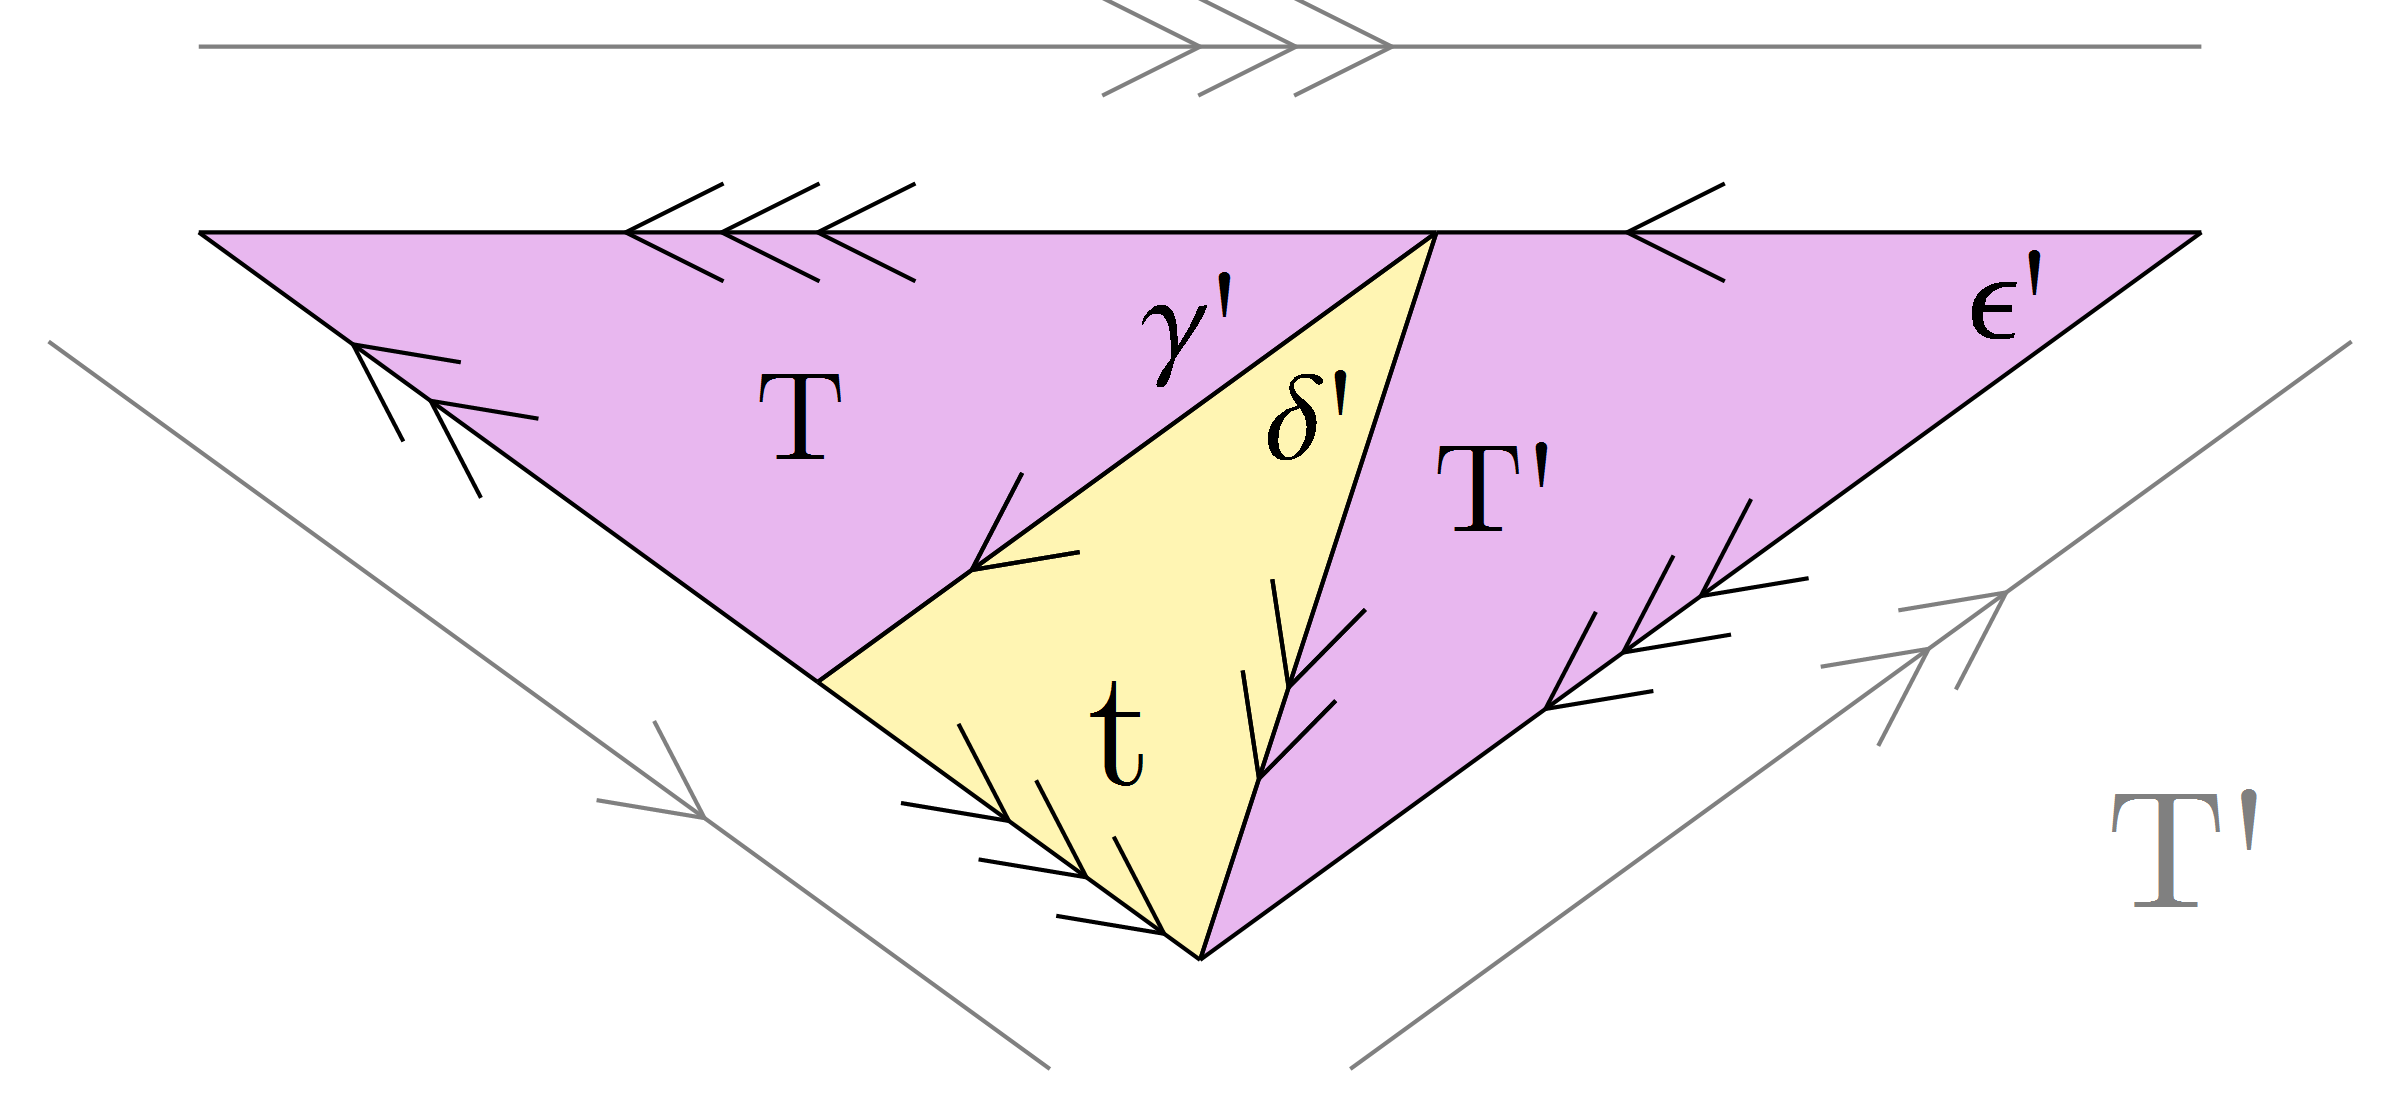
\includegraphics[width=\textwidth]{TF'}}
        \end{subfigure}\hfill
        \begin{subfigure}[t]{0.35\textwidth}
                \includegraphics[width=\textwidth]{TS'}
        \end{subfigure}   
        \caption{Oriented Robinson triangles with their constituent triangles. The relationship mappings between a constituent and parent triangles are given by lowercase Greek letters. For example, constituent triangle \textbf{T'} is related to parent triangle \textbf{T} under the mapping $\gamma$. The original edges of the parent triangles are also shown in grey. The relationship between the constituent and parent edges is shown in Fig.\ref{fig:EdgeRules}.}
        \label{fig:OrientedSub}                     
\end{figure}

From these mappings we can see why the explicit description of triangle orientation is necessary here. Otherwise, for instance, it would be ambiguous which constituent thick triangle, \textbf{T} or \textbf{T'}, we are describing inside a parent \textbf{T}.

We can alternatively visualize the mappings in Equations (\ref{eq:maps}) as directed graphs embedding constituent triangles into parent triangles, see Fig.\ref{fig:functionmap}. 

\begin{figure}[H]
        \begin{subfigure}[t]{0.6\textwidth}
                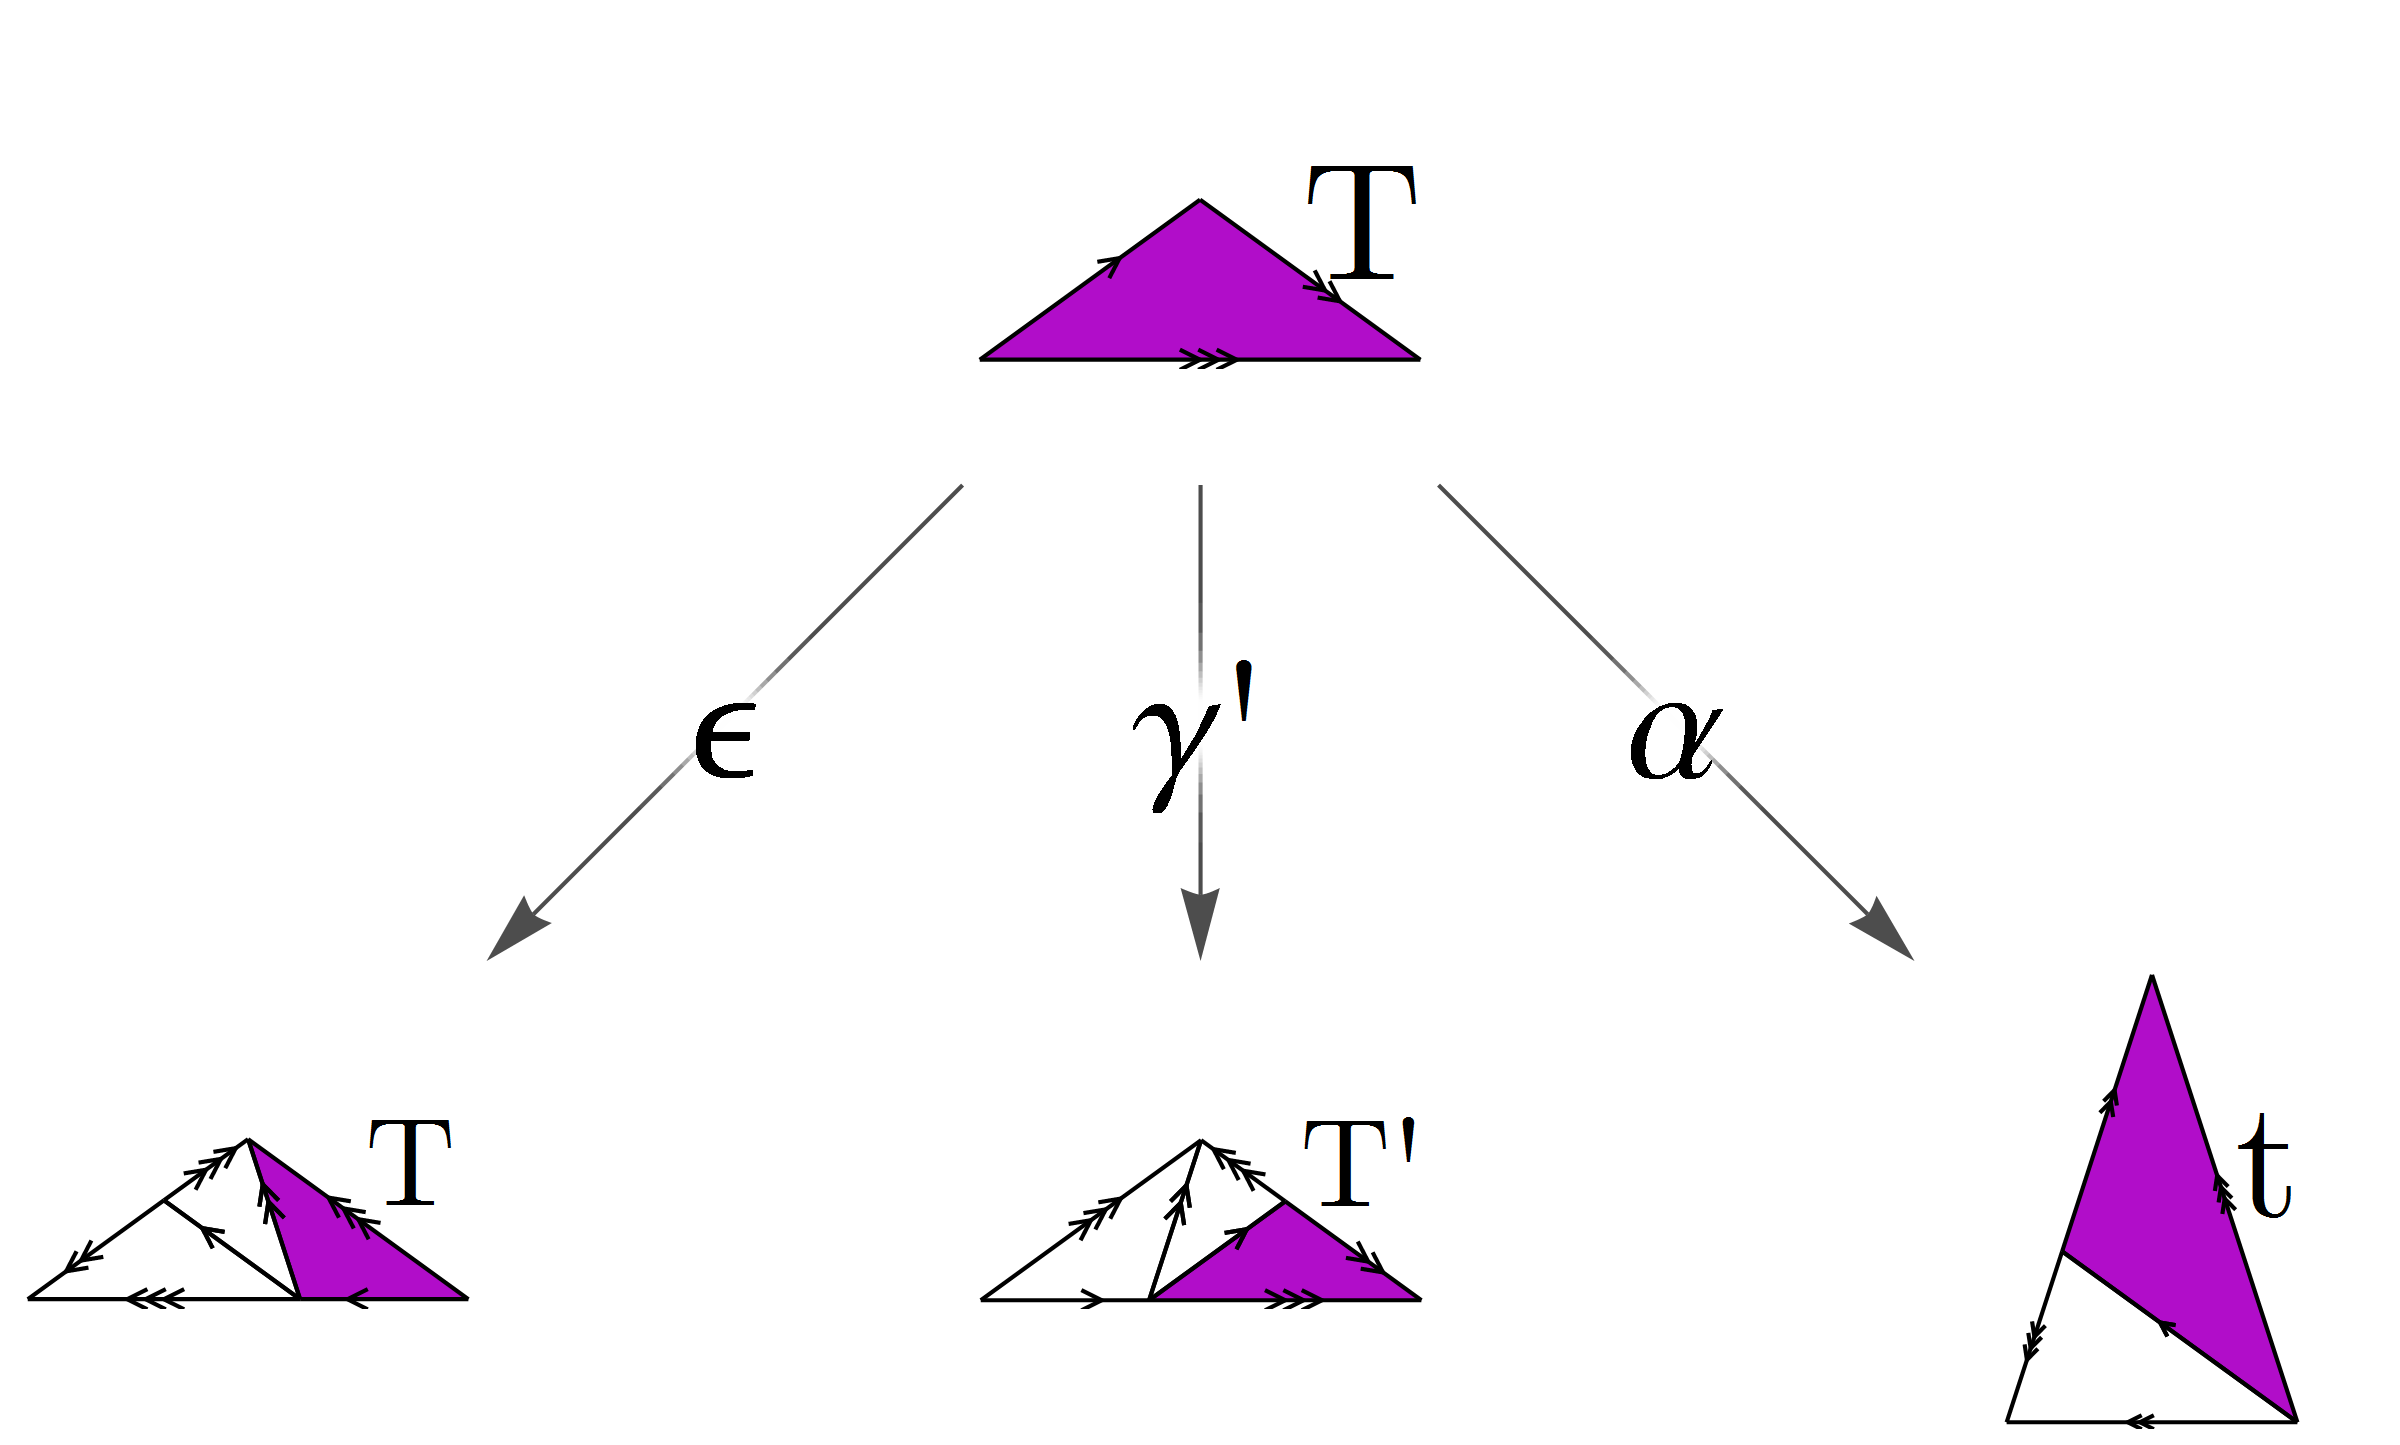
\includegraphics[width=\textwidth]{TRgraph}
        \end{subfigure}\hfill
        \begin{subfigure}[t]{0.4\textwidth}
                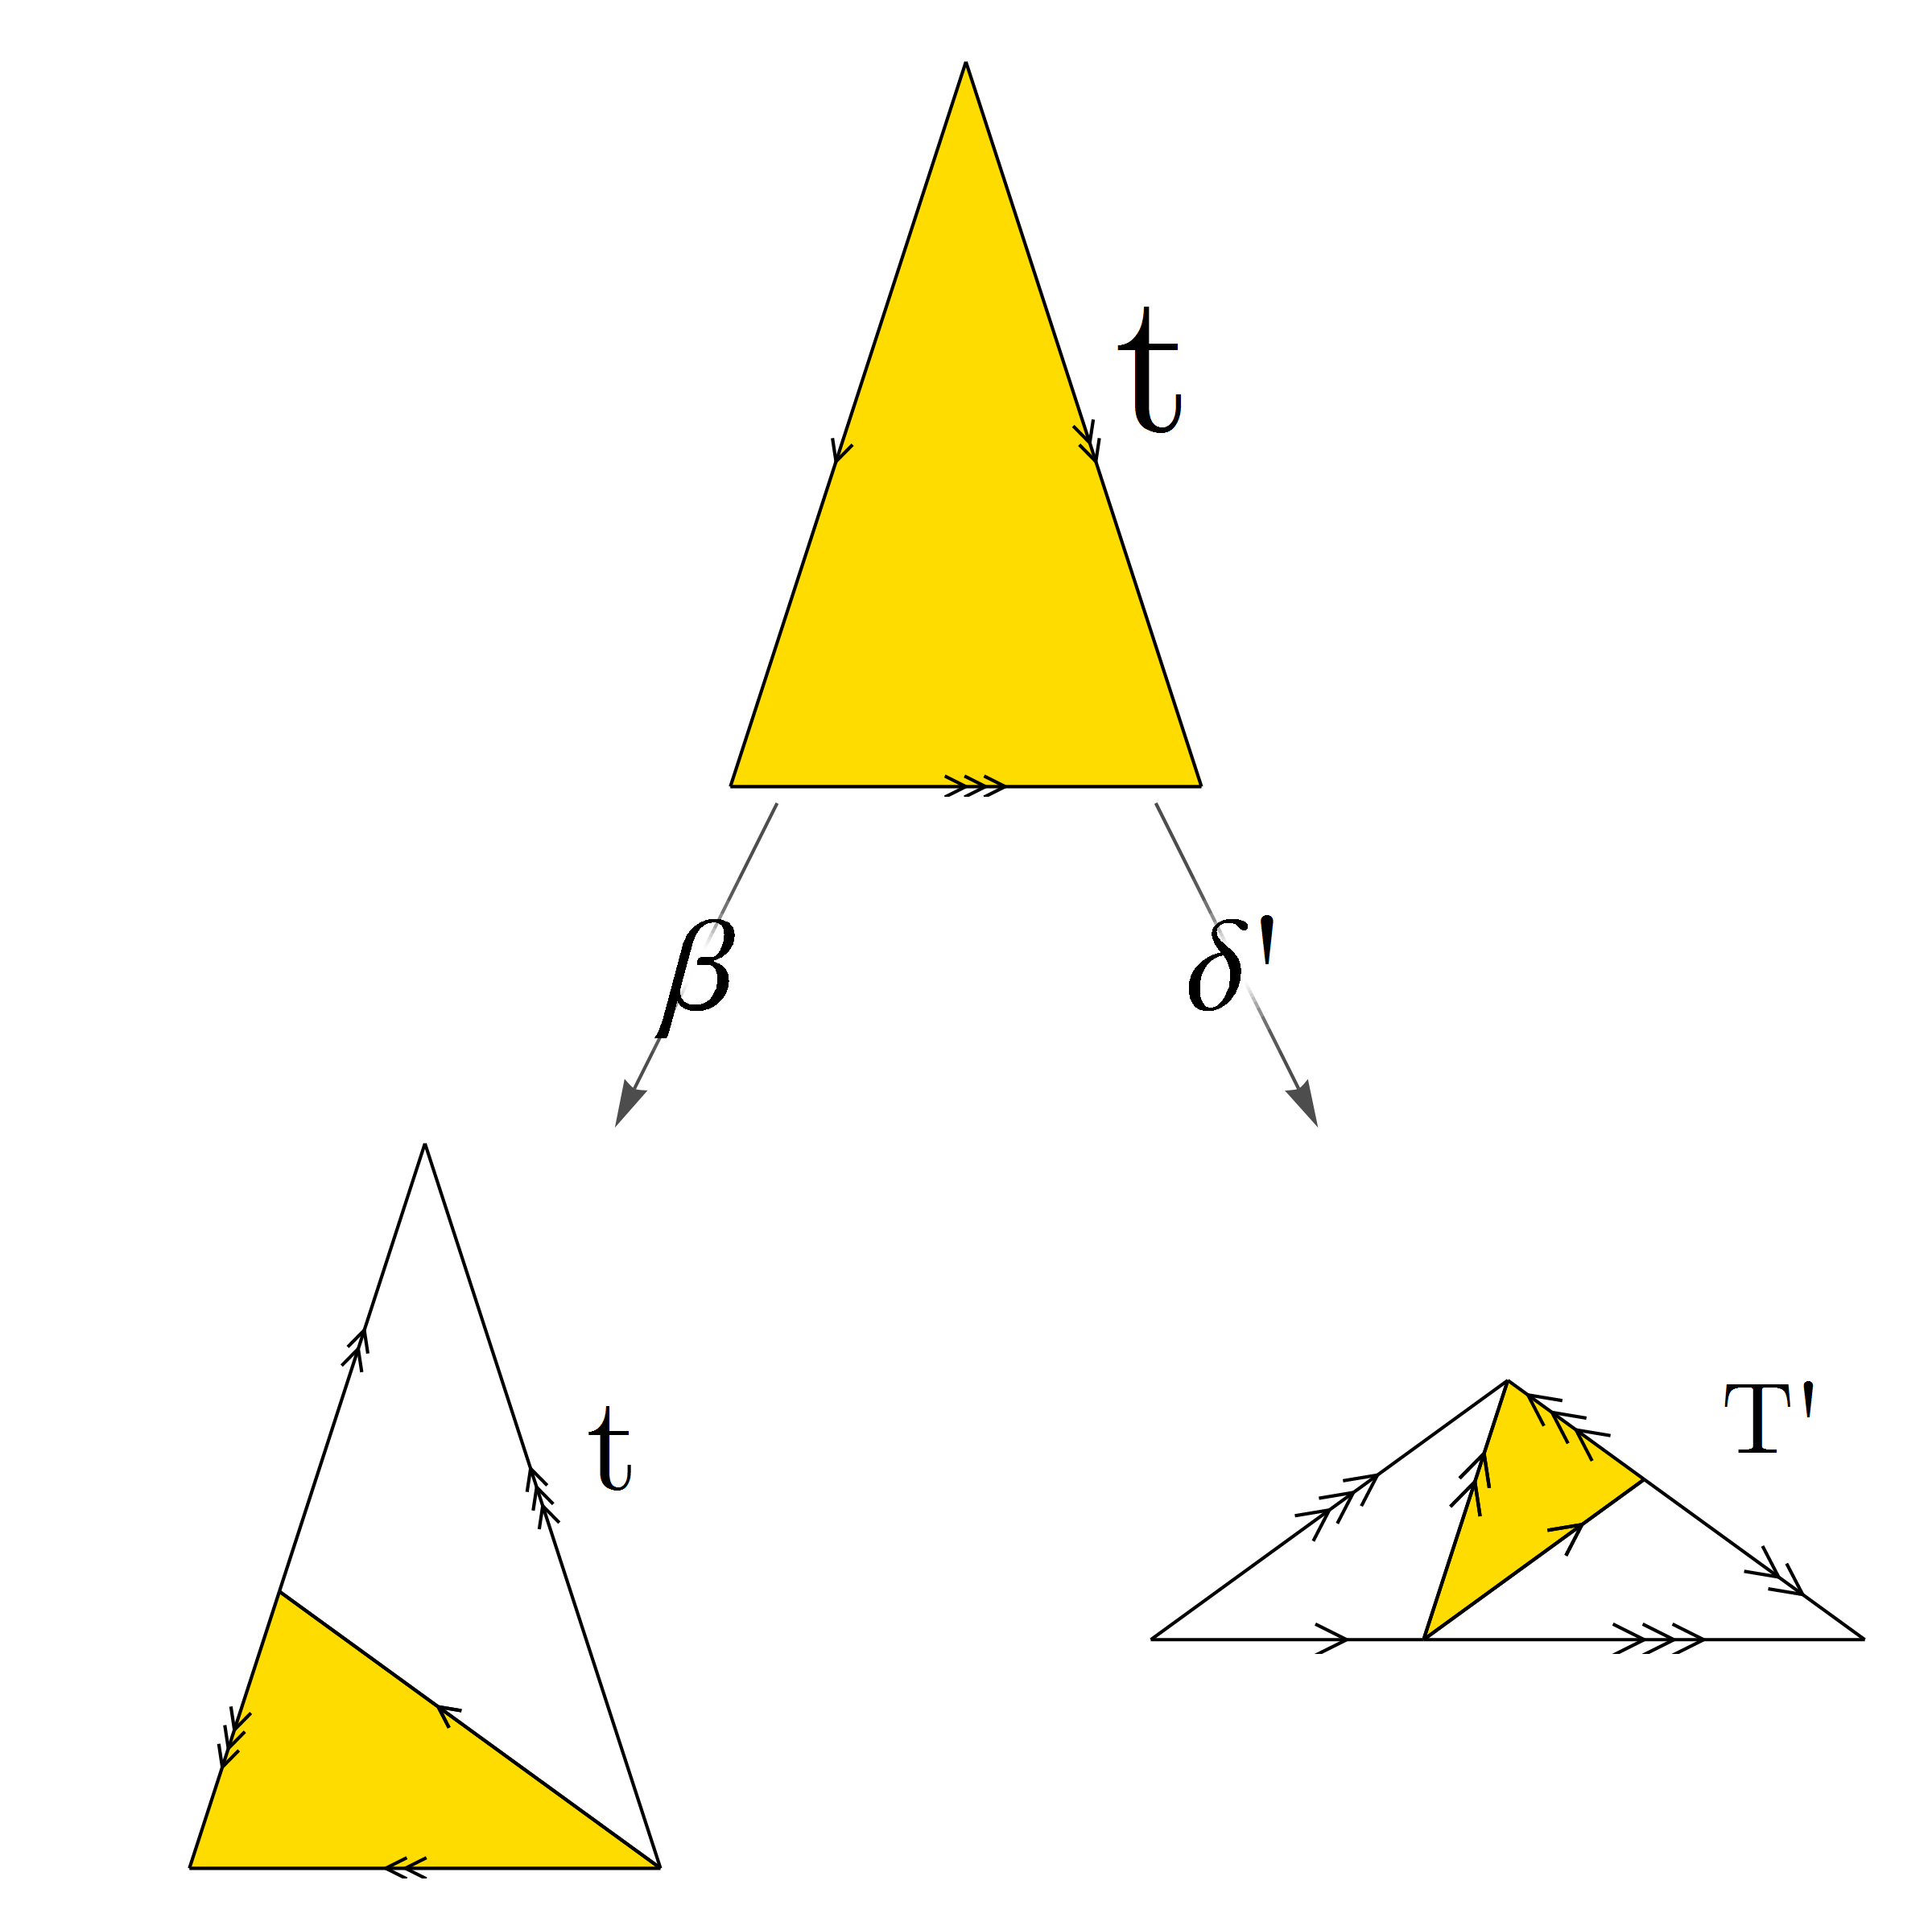
\includegraphics[width=\textwidth]{tsrgraph}
        \end{subfigure}\\
        
        \begin{subfigure}[t]{0.6\textwidth}
                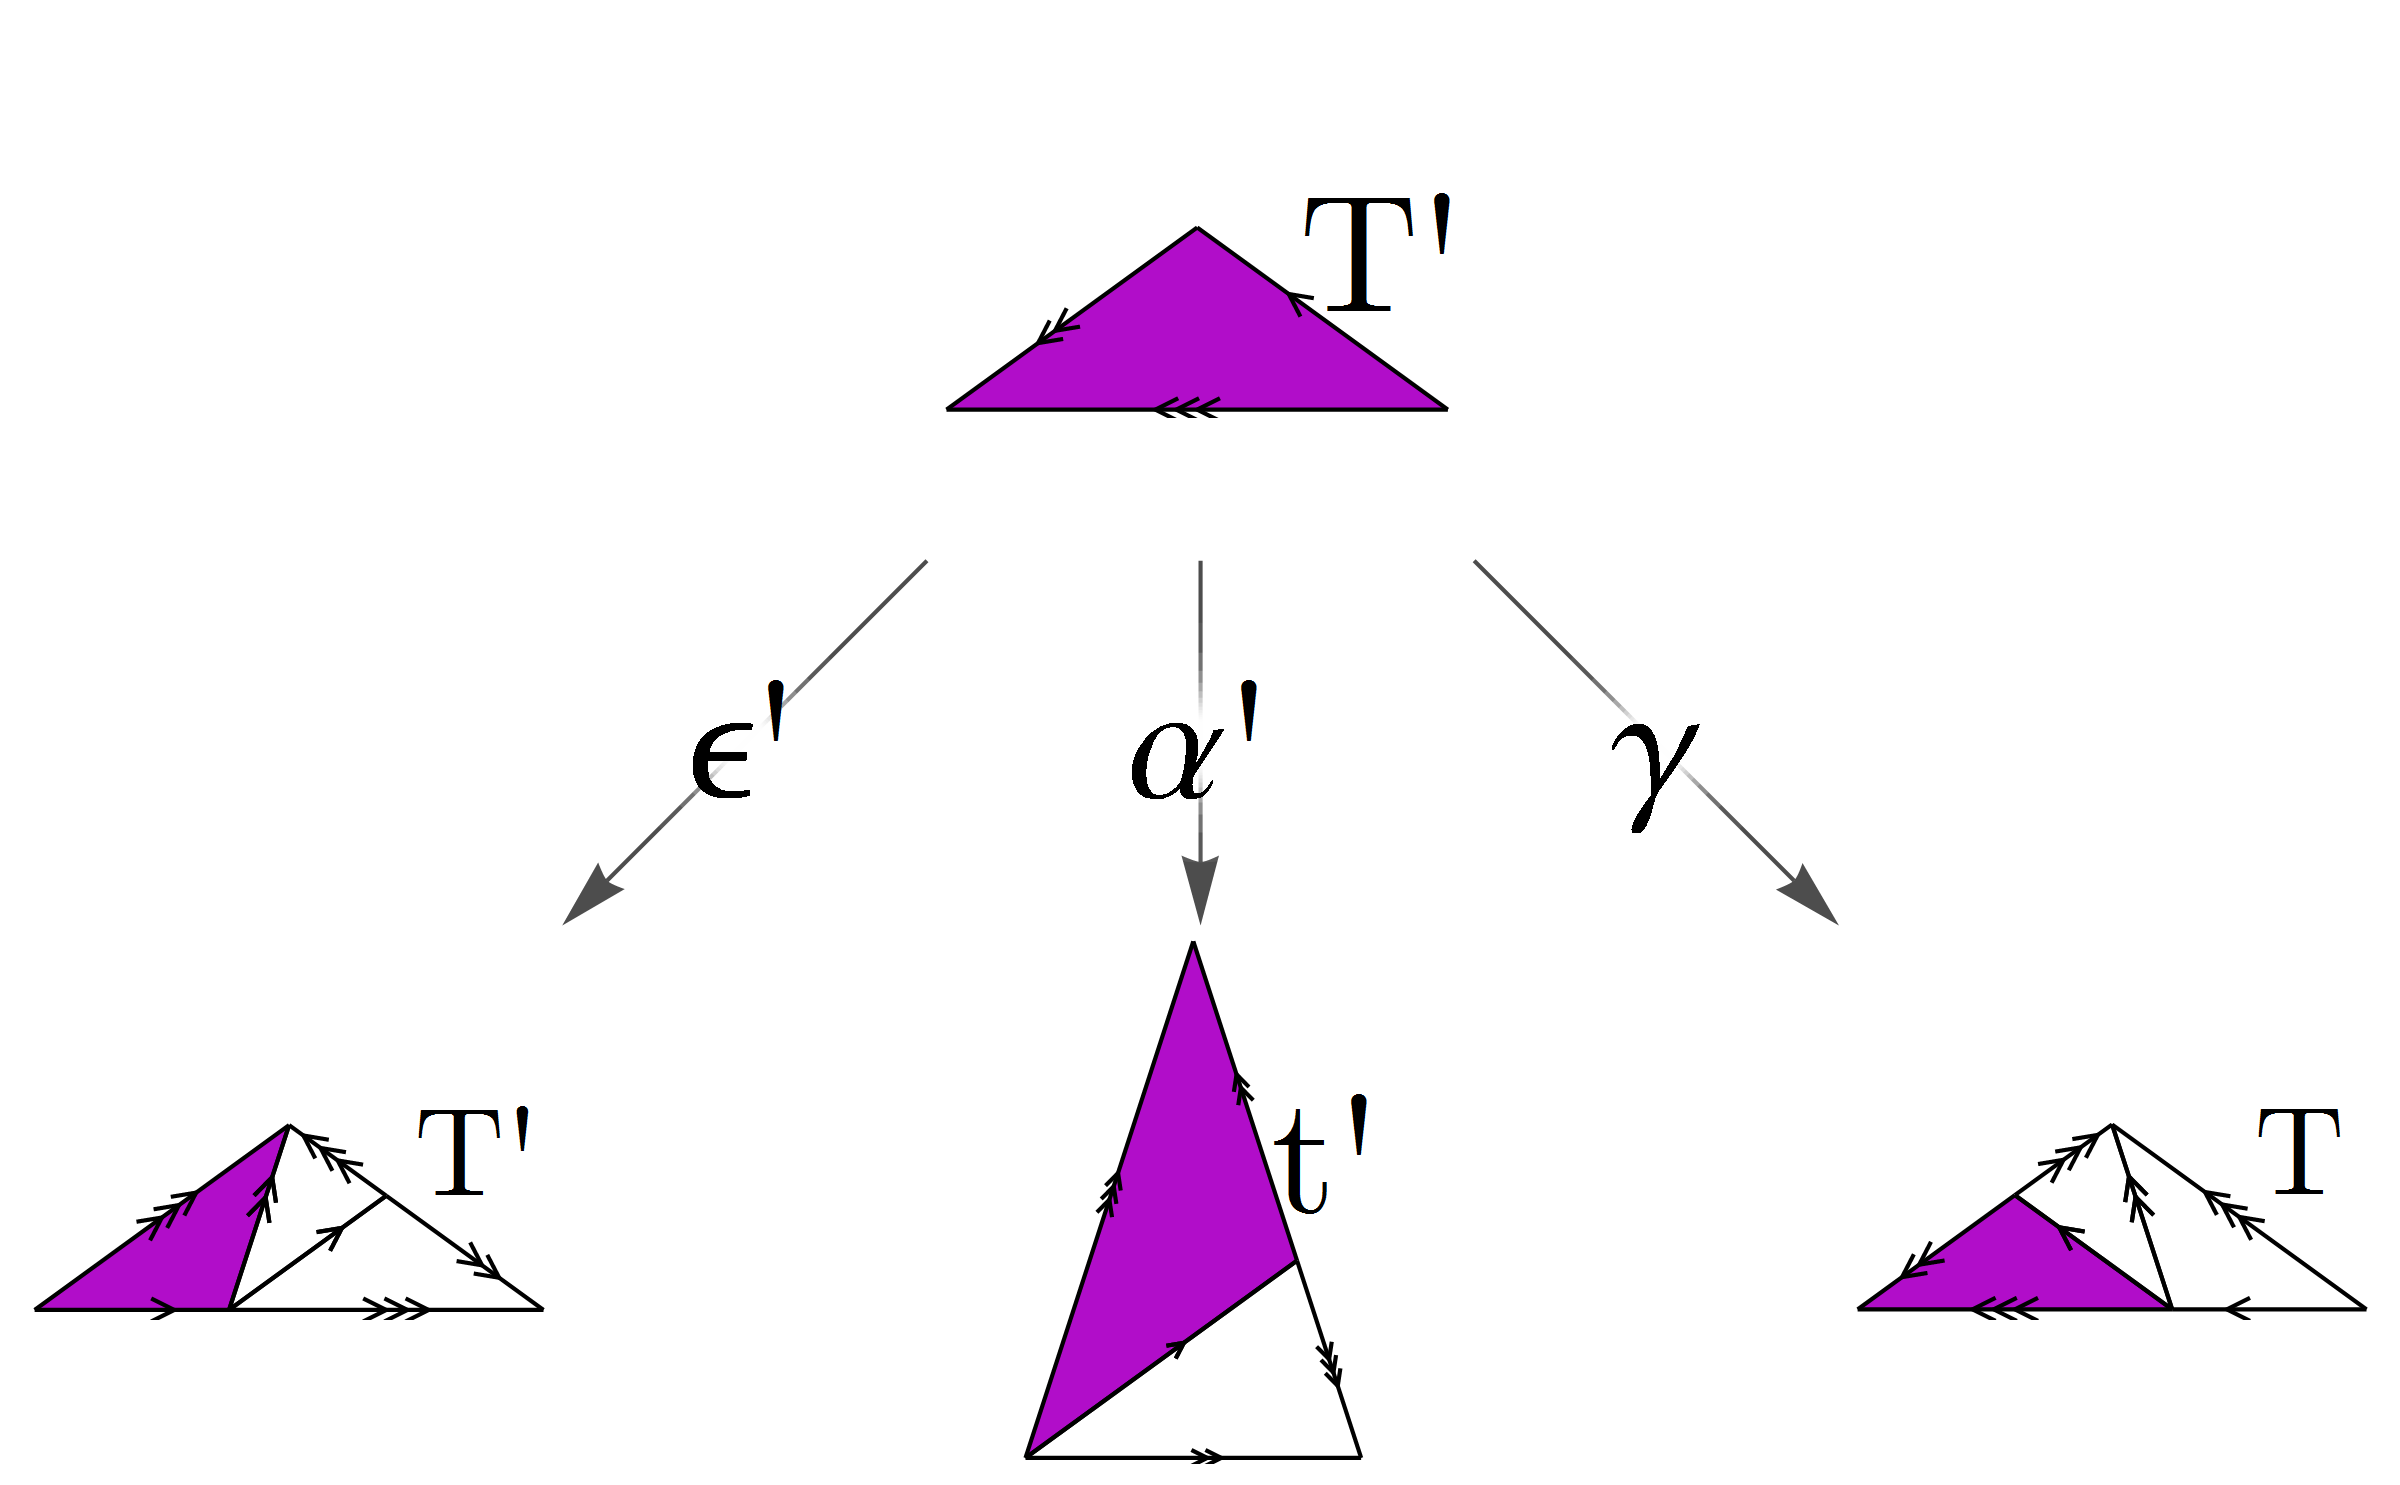
\includegraphics[width=\textwidth]{TLgraph}
        \end{subfigure}\hfill
        \begin{subfigure}[t]{0.4\textwidth}
                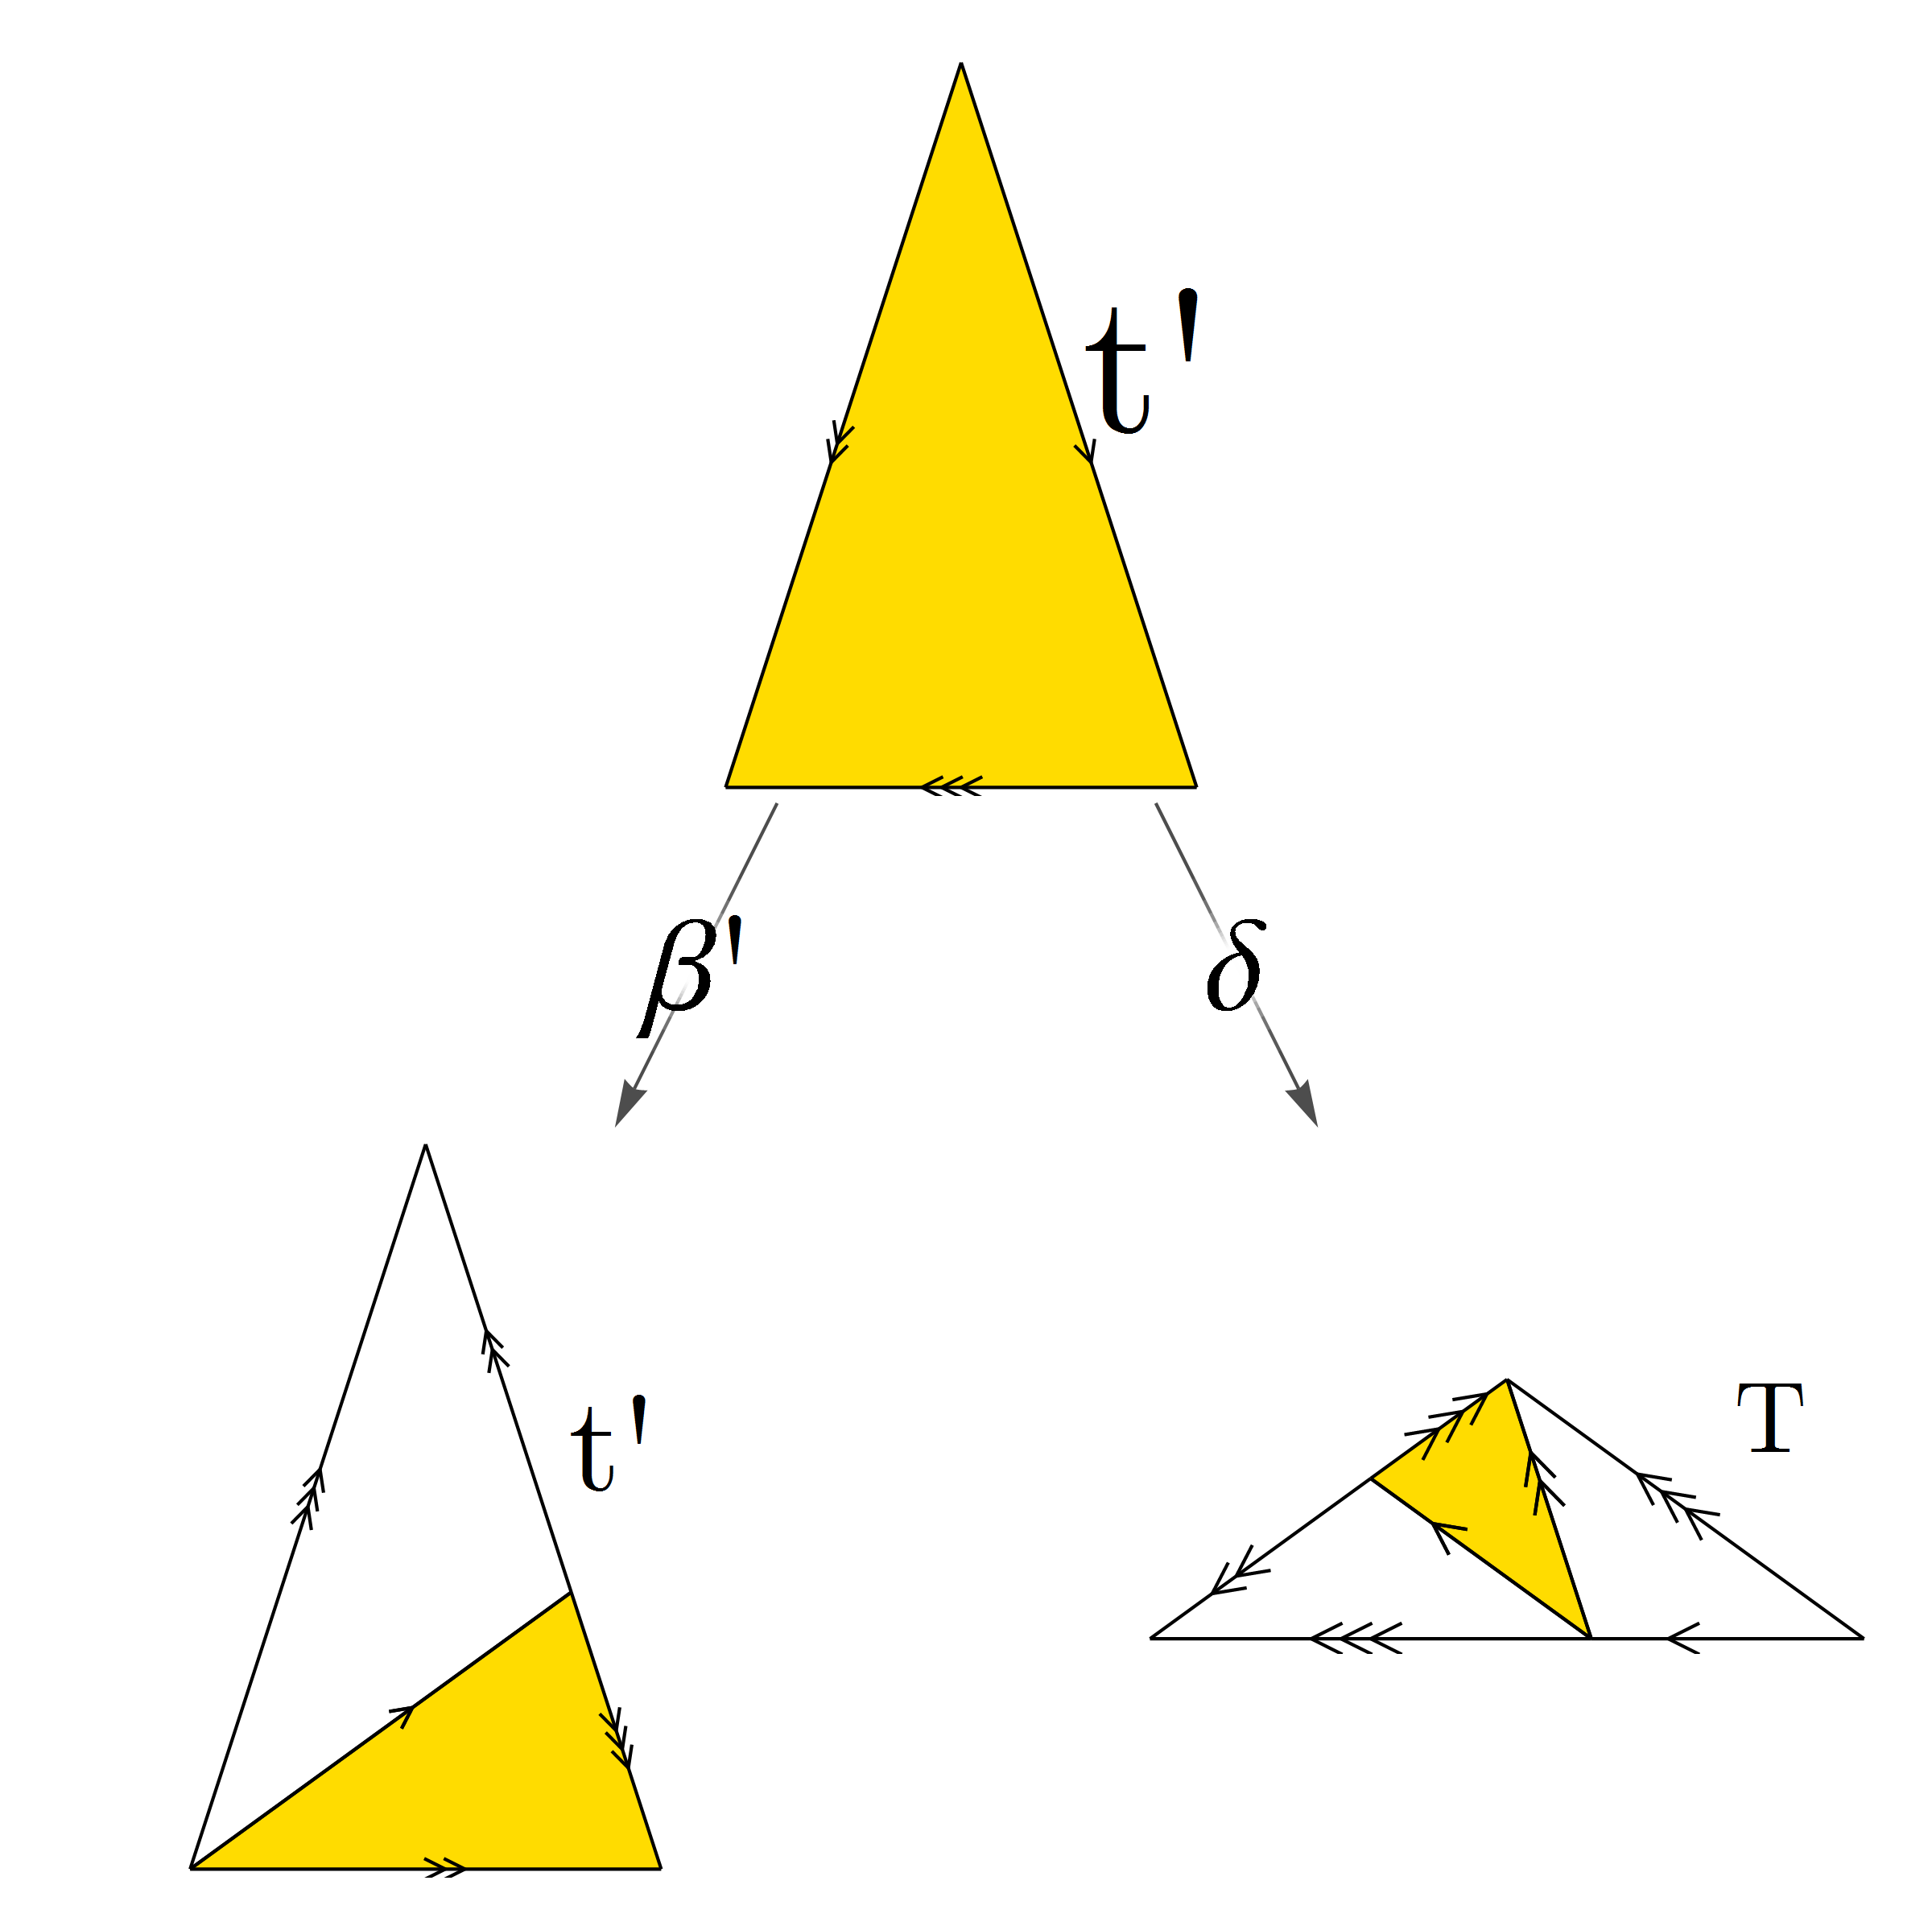
\includegraphics[width=\textwidth]{tslgraph}
        \end{subfigure}  
        \caption{Relationship mapping from constituent triangles to parent triangles given by Equations (\ref{eq:maps})} 
        \label{fig:functionmap}                    
\end{figure}

We are now ready to introduce the Up process. Realizing that mappings from Equations (\ref{eq:maps}) will place constituent triangles inside parent triangles, we see that each application of a mapping will generate a larger finite region of the tiling. Think of this process as the opposite of substitution, we are starting from a constituent and generating a substituted parent triangle. Just as substitution generated a finite section of a tiling, by mapping a constituent to a substituted parent triangle we have similarly generated a finite section.

Further, just as with the substitution method, the end result of each mapping is an oriented Robinson triangle. That is, the image of every mapping will be the domain of other mappings. This allows us to form compositions of the mappings, from the image of one to the domain of another. To illustrate how these mappings can be composed from another, we have a directed graph in Fig.\ref{fig:UpDownGraph}.

\begin{figure}[H]
\centering
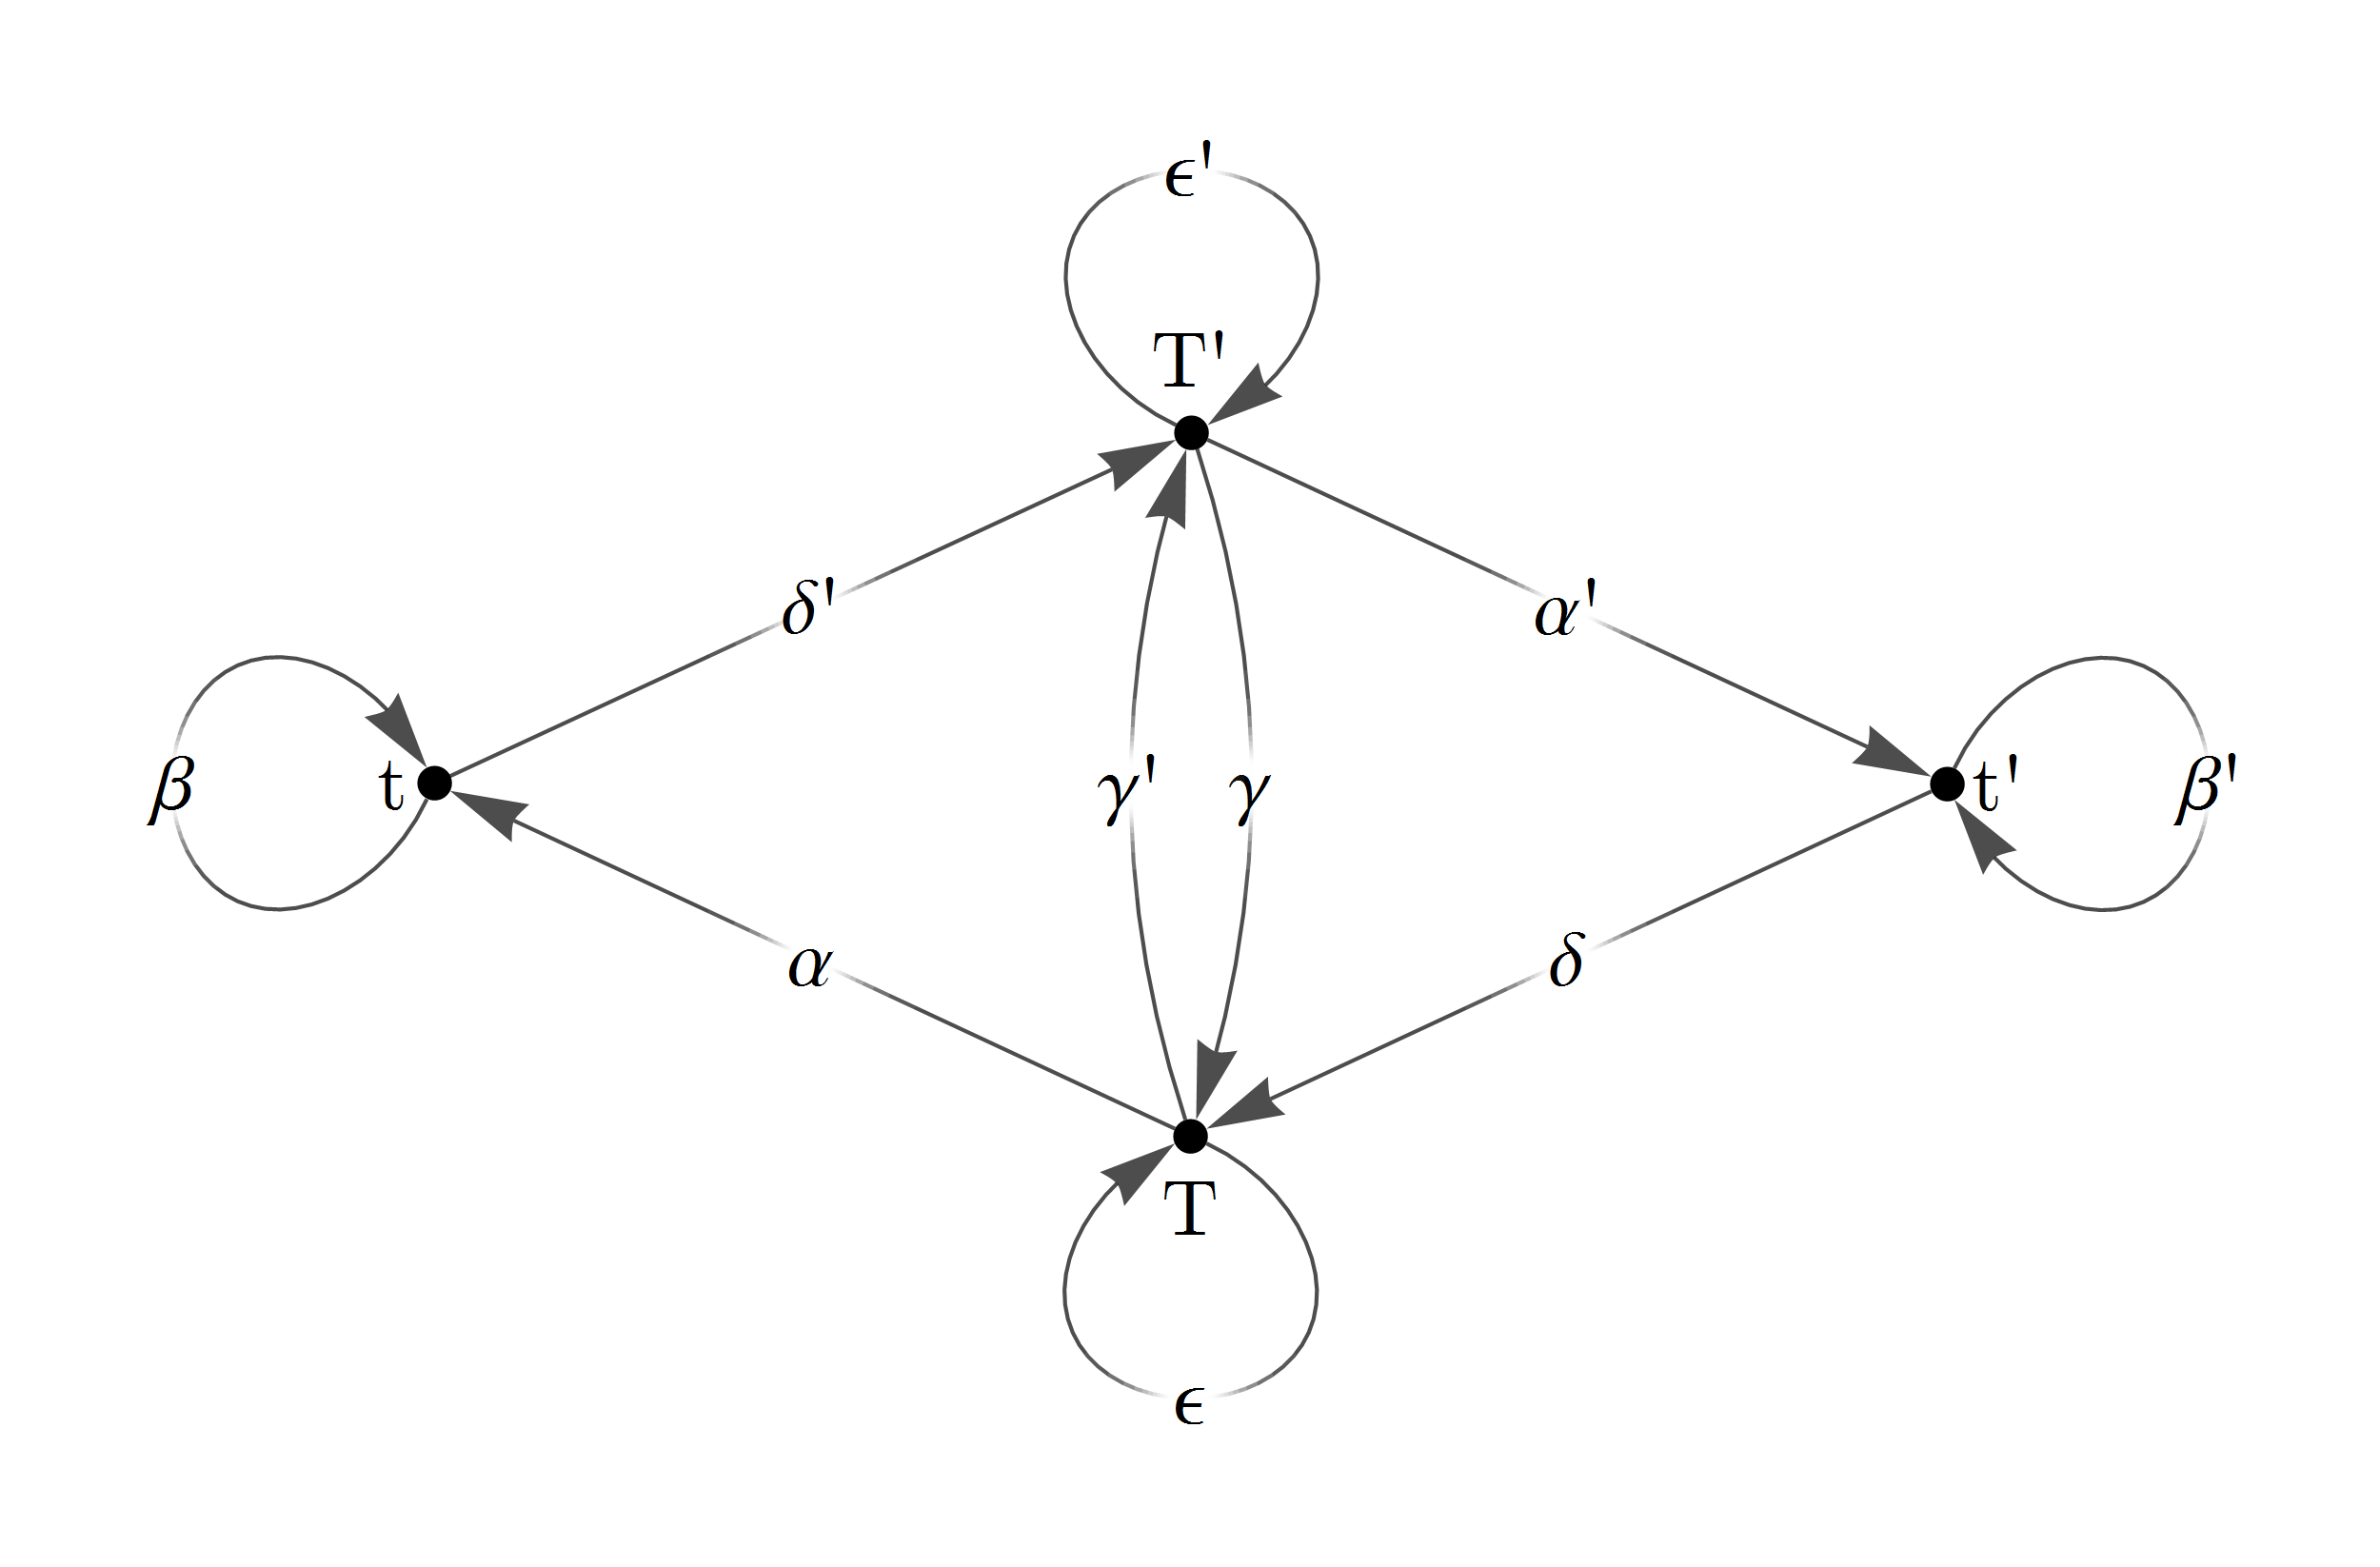
\includegraphics[width=\textwidth]{UpDownGraph}
\caption{A directed graph, or finite automaton, for the generation of parent triangles from constituent triangles. Paths along the directed edges represent compositions of the mappings from Equations (\ref{eq:maps}). Infinite paths along the directed edges may generate Penrose tilings of the plane.}
\label{fig:UpDownGraph}
\end{figure}

Finite paths along this directed graph will generate finite subregions of a Penrose tiling. Infinite paths along this directed graph will generate tilings of the plane, half-plane, or $\frac{\pi}{5}$-plane wedge. The $\frac{\pi}{5}$-plane wedge will be discussed later, as Penrose tilings generated from such infinite paths will exhibit five-fold rotational symmetry about a single point. 


\begin{center}
\begin{tabular}{ccc}
\raisebox{0px}{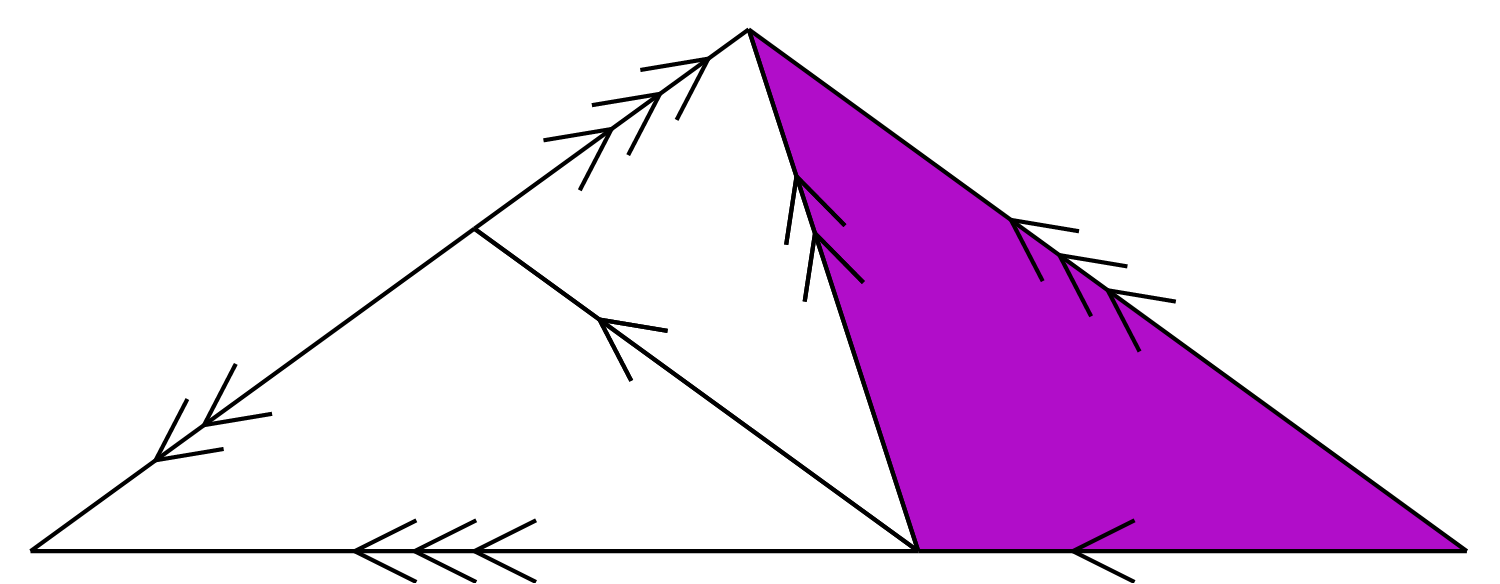
\includegraphics[width=0.3\textwidth]{Up4Left}} & \raisebox{50px}{\Large \textcolor{gray}{$ \rightarrow$}} & 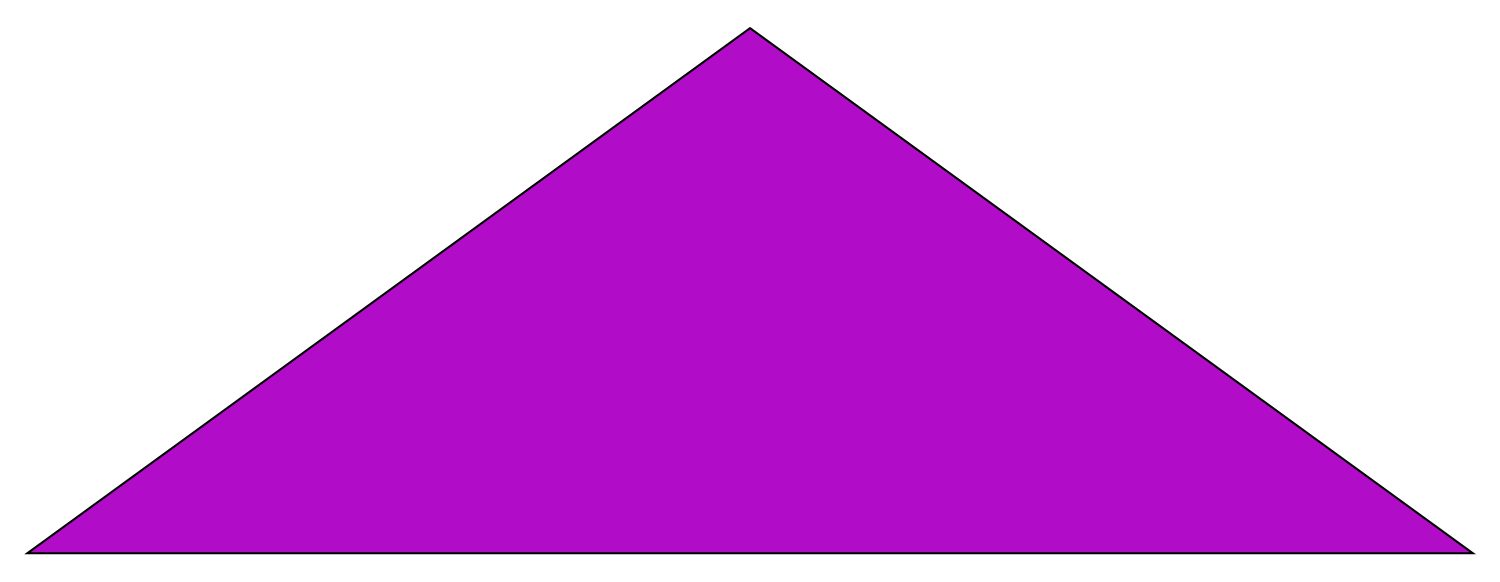
\includegraphics[width=0.6\textwidth]{Down4}\\
\Large $\uparrow$ $\epsilon$ & \hfill & $\downarrow$\\ 
\raisebox{0px}{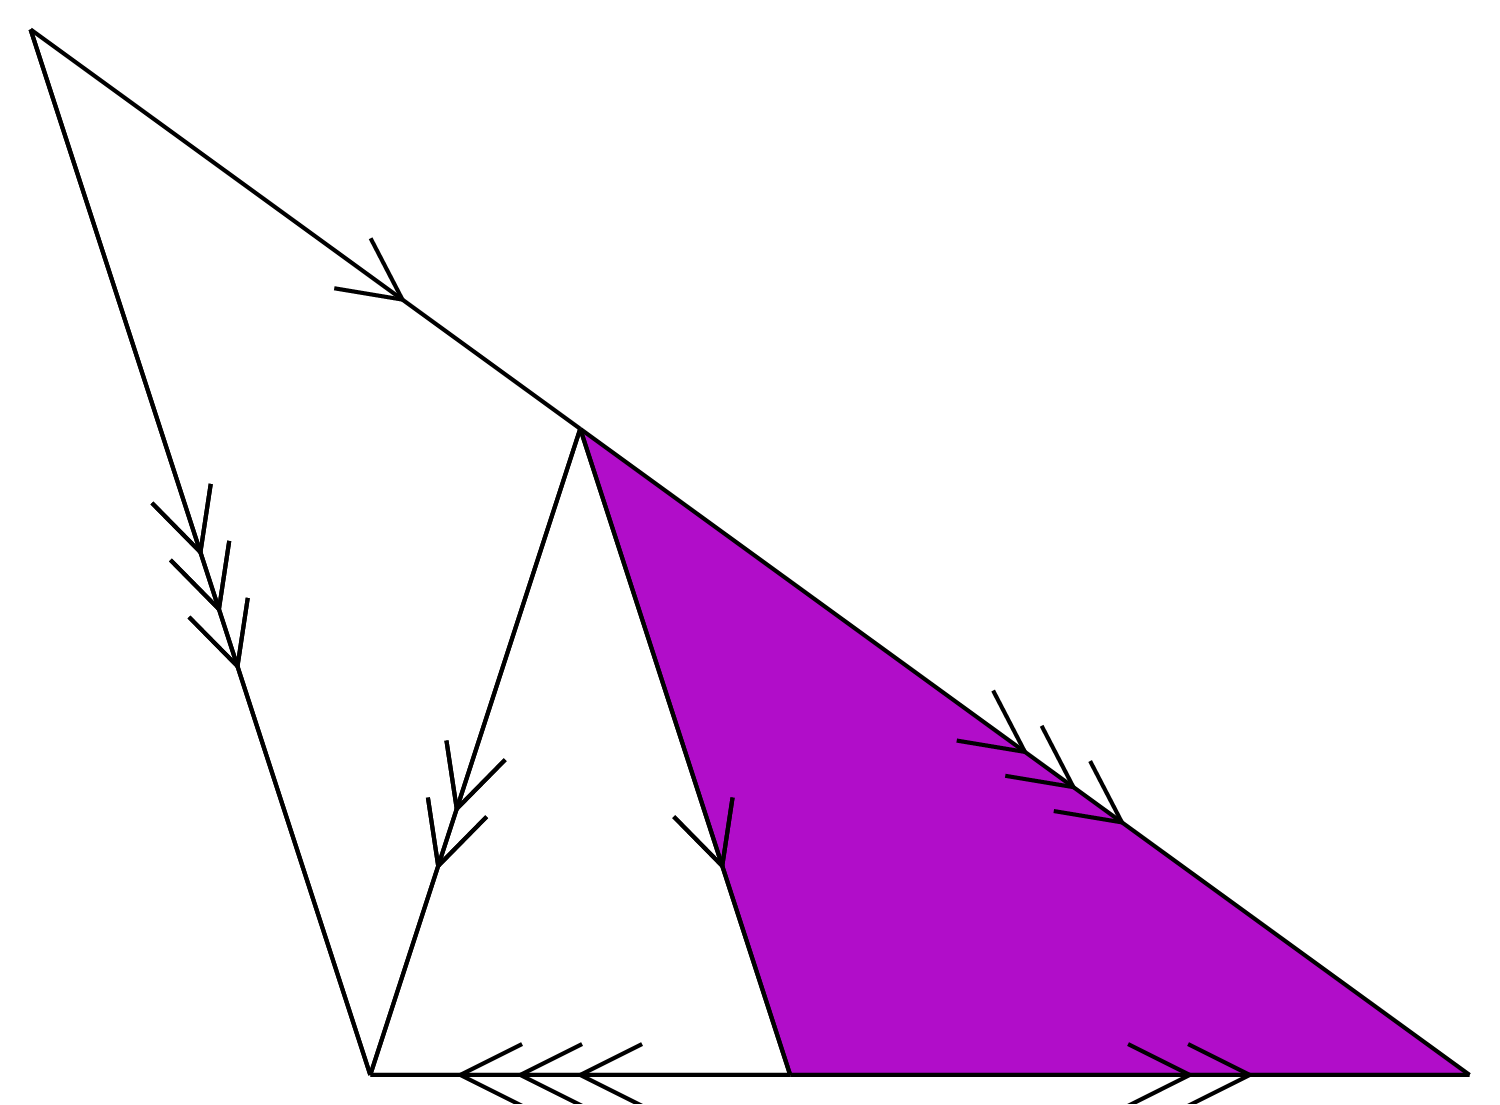
\includegraphics[width=0.3\textwidth]{Up3Left}} & \raisebox{50px}{\Large \textcolor{gray}{$ \rightarrow$}} & 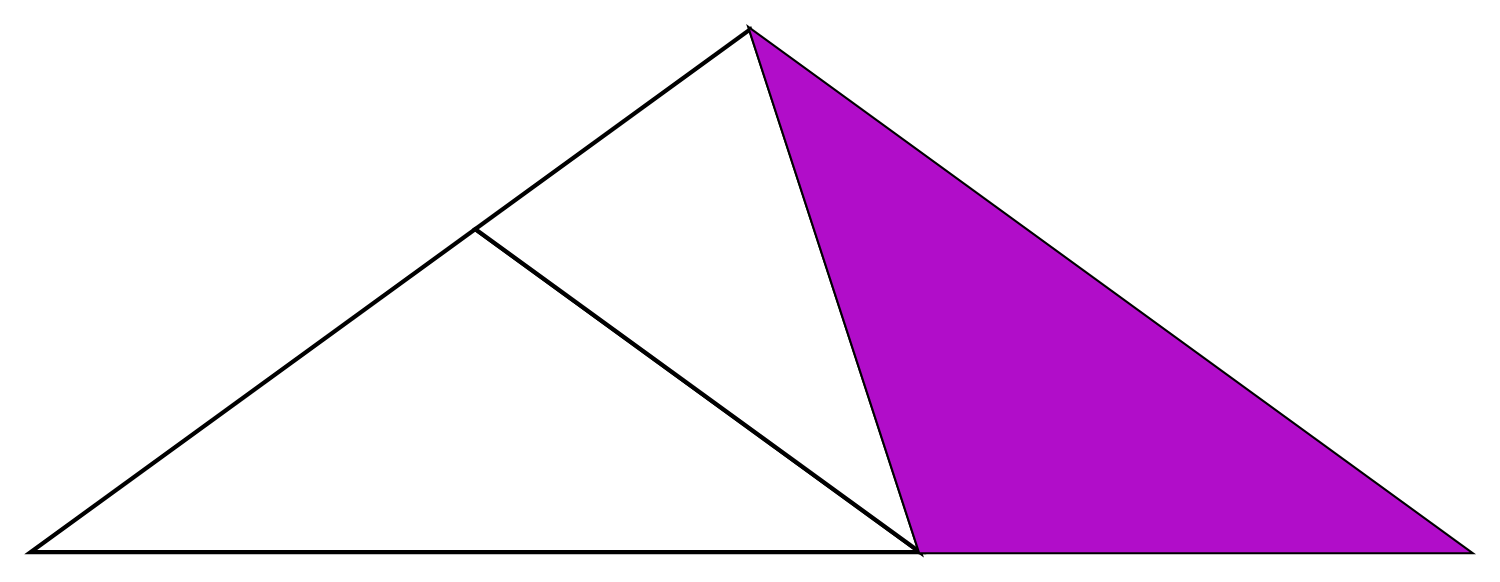
\includegraphics[width=0.6\textwidth]{Down3}\\
\Large $\uparrow$ $\gamma$ & \hfill & $\downarrow$\\ 
\raisebox{0px}{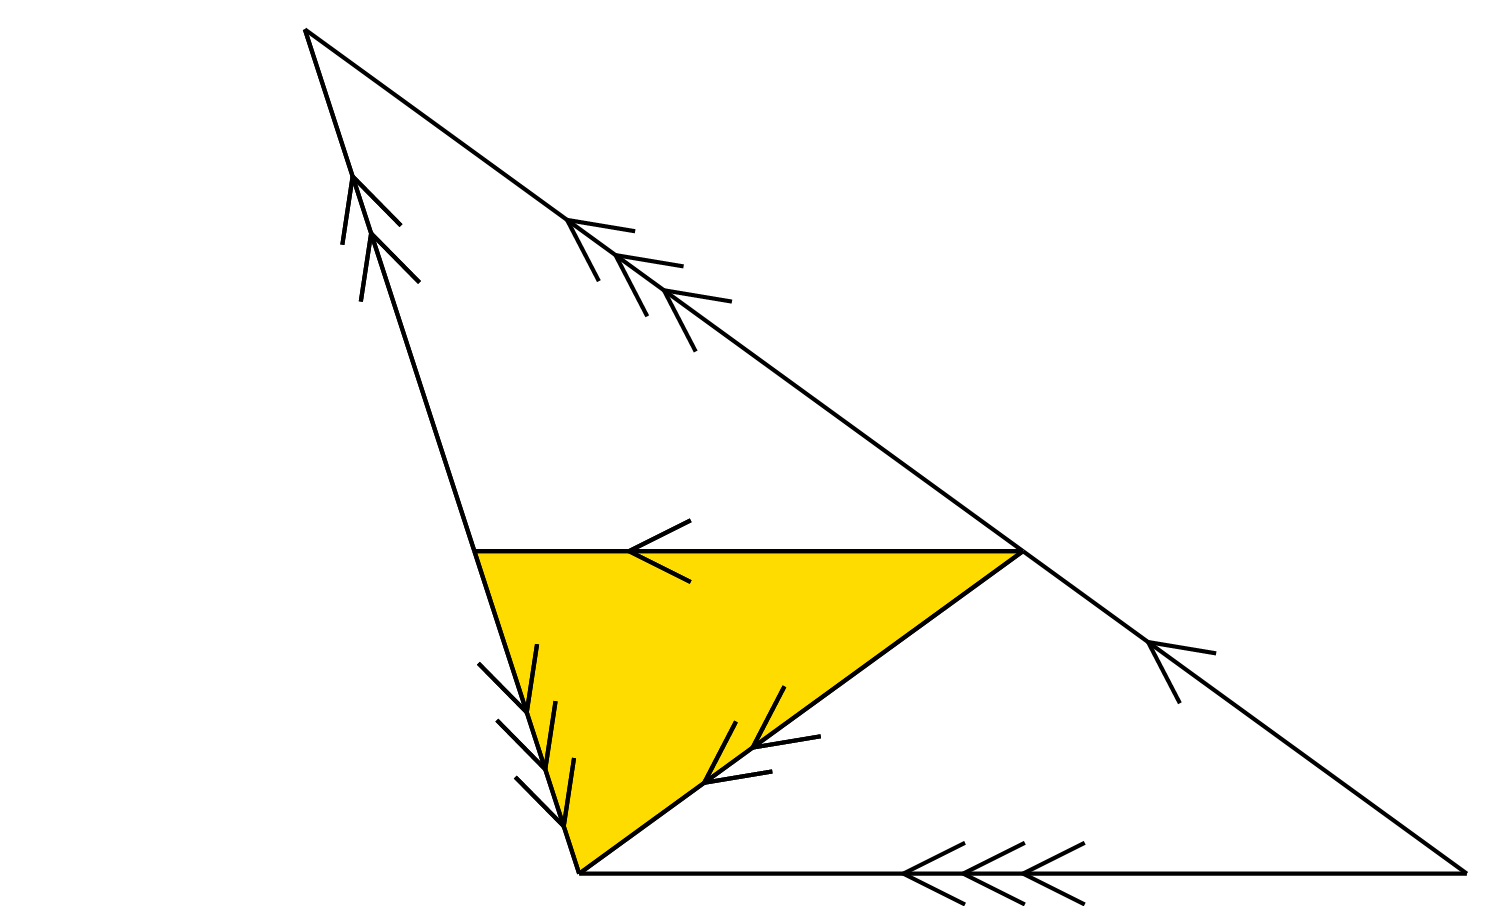
\includegraphics[width=0.4\textwidth]{Up2Left}} & \raisebox{50px}{\Large \textcolor{gray}{$ \rightarrow$}} & 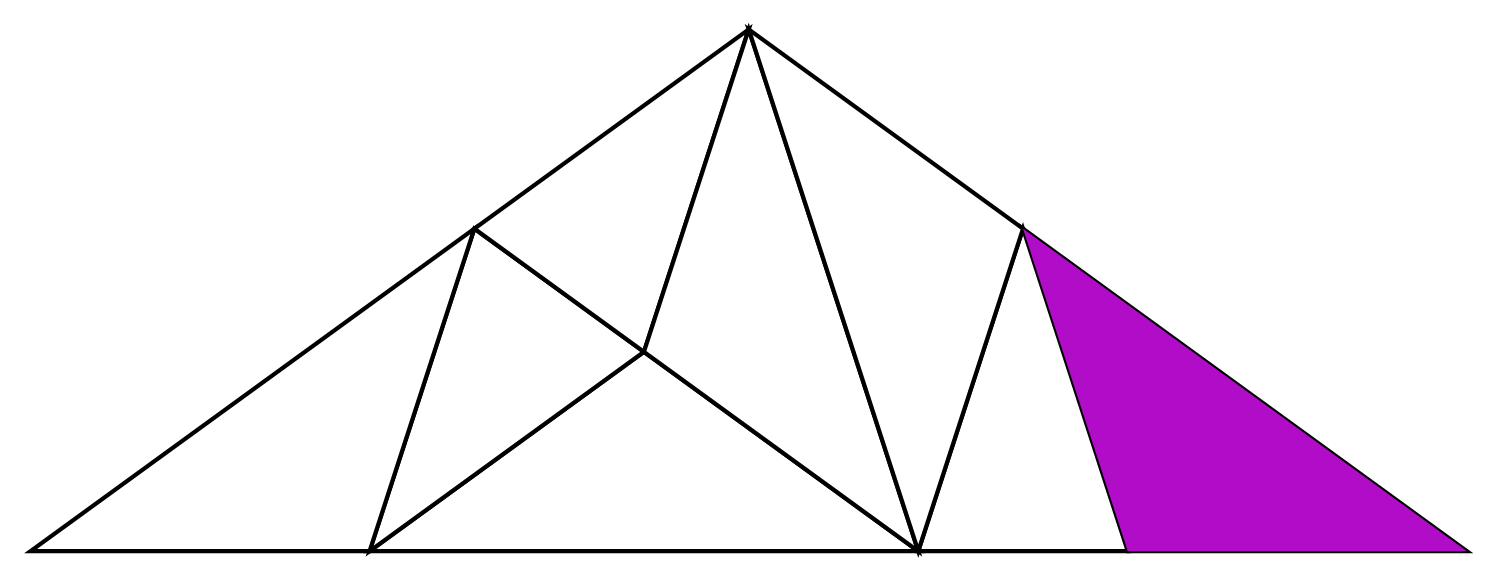
\includegraphics[width=0.6\textwidth]{Down2}\\
\Large $\uparrow$ $\delta'$ & \hfill & $\downarrow$\\ 
\raisebox{0px}{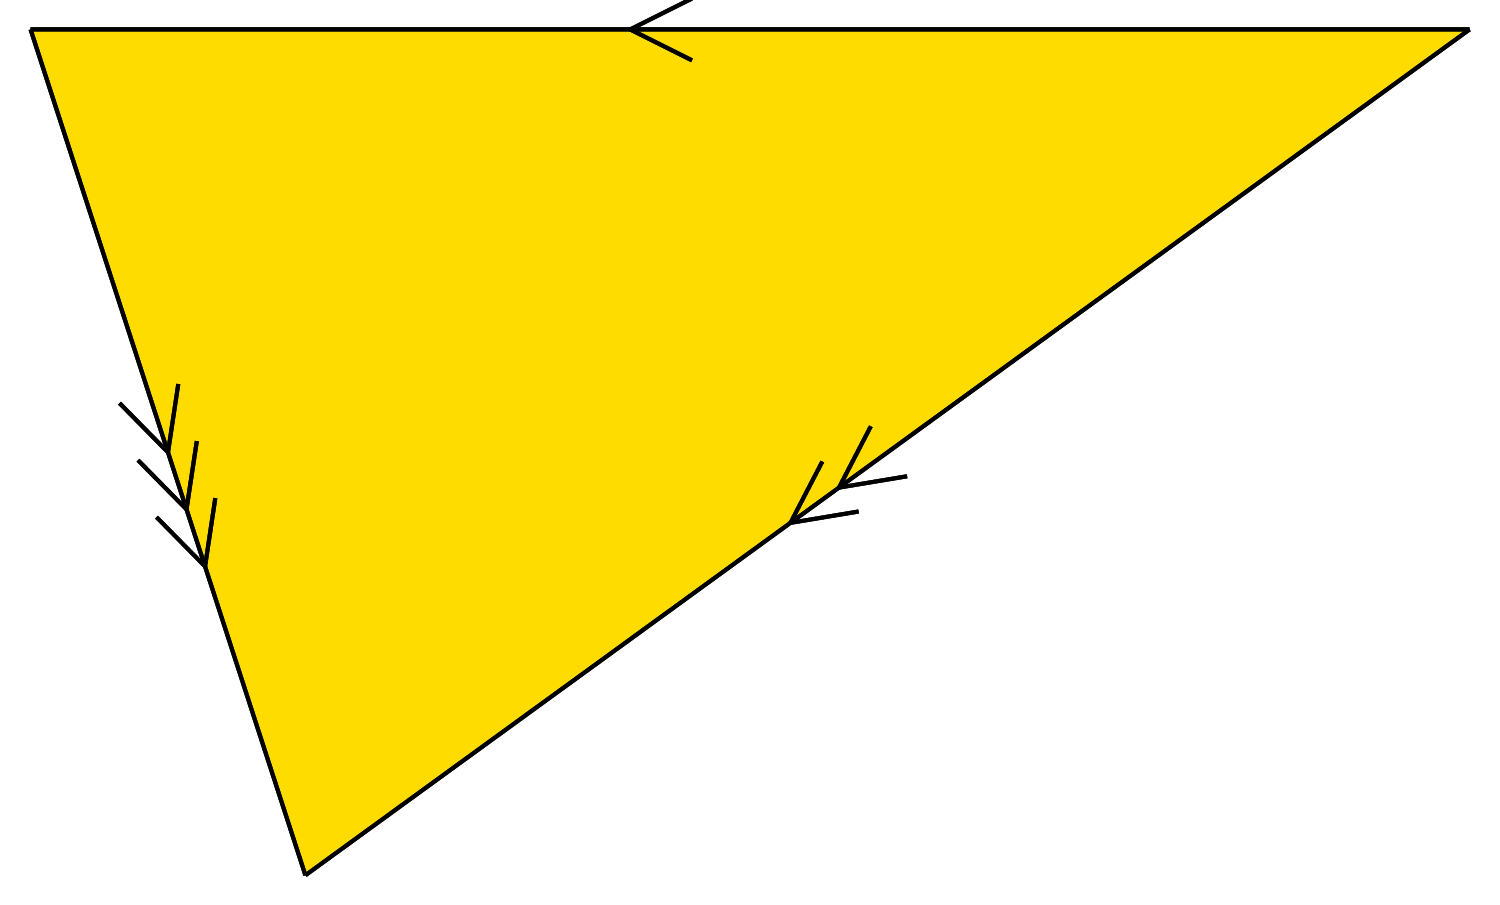
\includegraphics[width=0.3\textwidth]{Up1Left}} &\raisebox{50px}{\Large \textcolor{gray}{$ \rightarrow$}}& 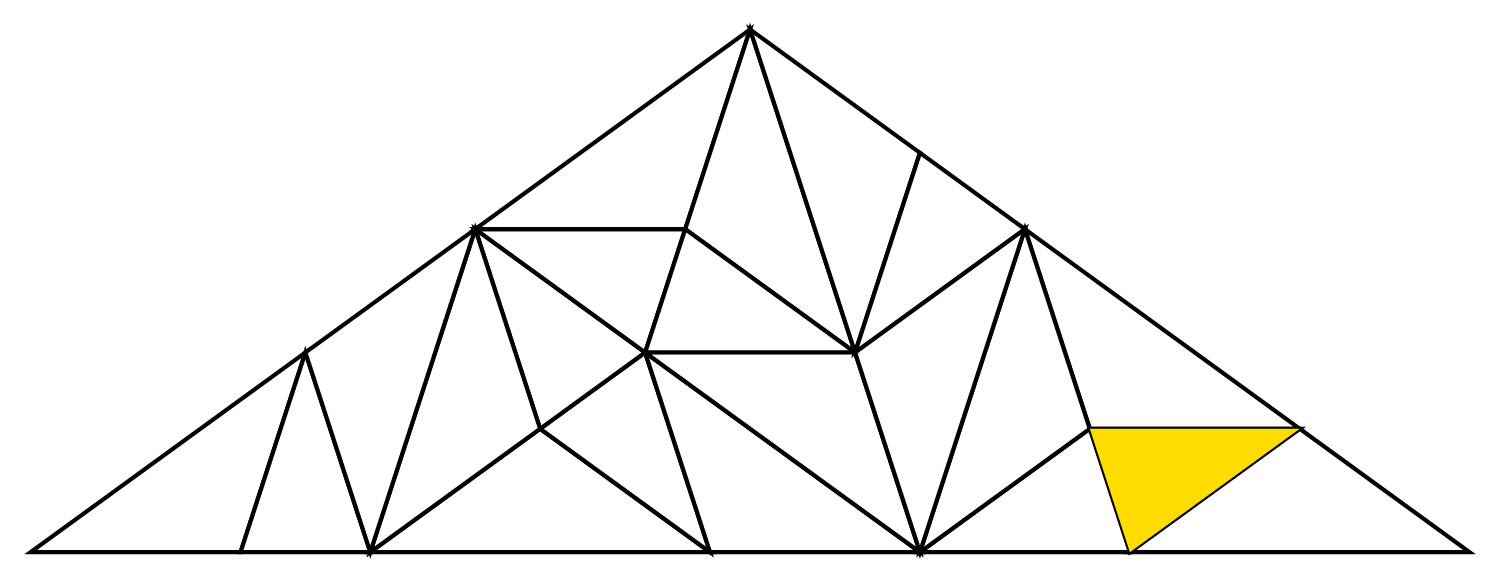
\includegraphics[width=0.6\textwidth]{Down1}\\
\end{tabular}
\end{center}


 
\subsection{Unaccountability of Tilings}

\end{document}